
% \begin{frame}[t]  \frametitle{Selecting mono-top events}
%   \vspace{-5mm}
%   \begin{columns}[T]
%   \begin{column}{0.5\textwidth}
%   \centering
%     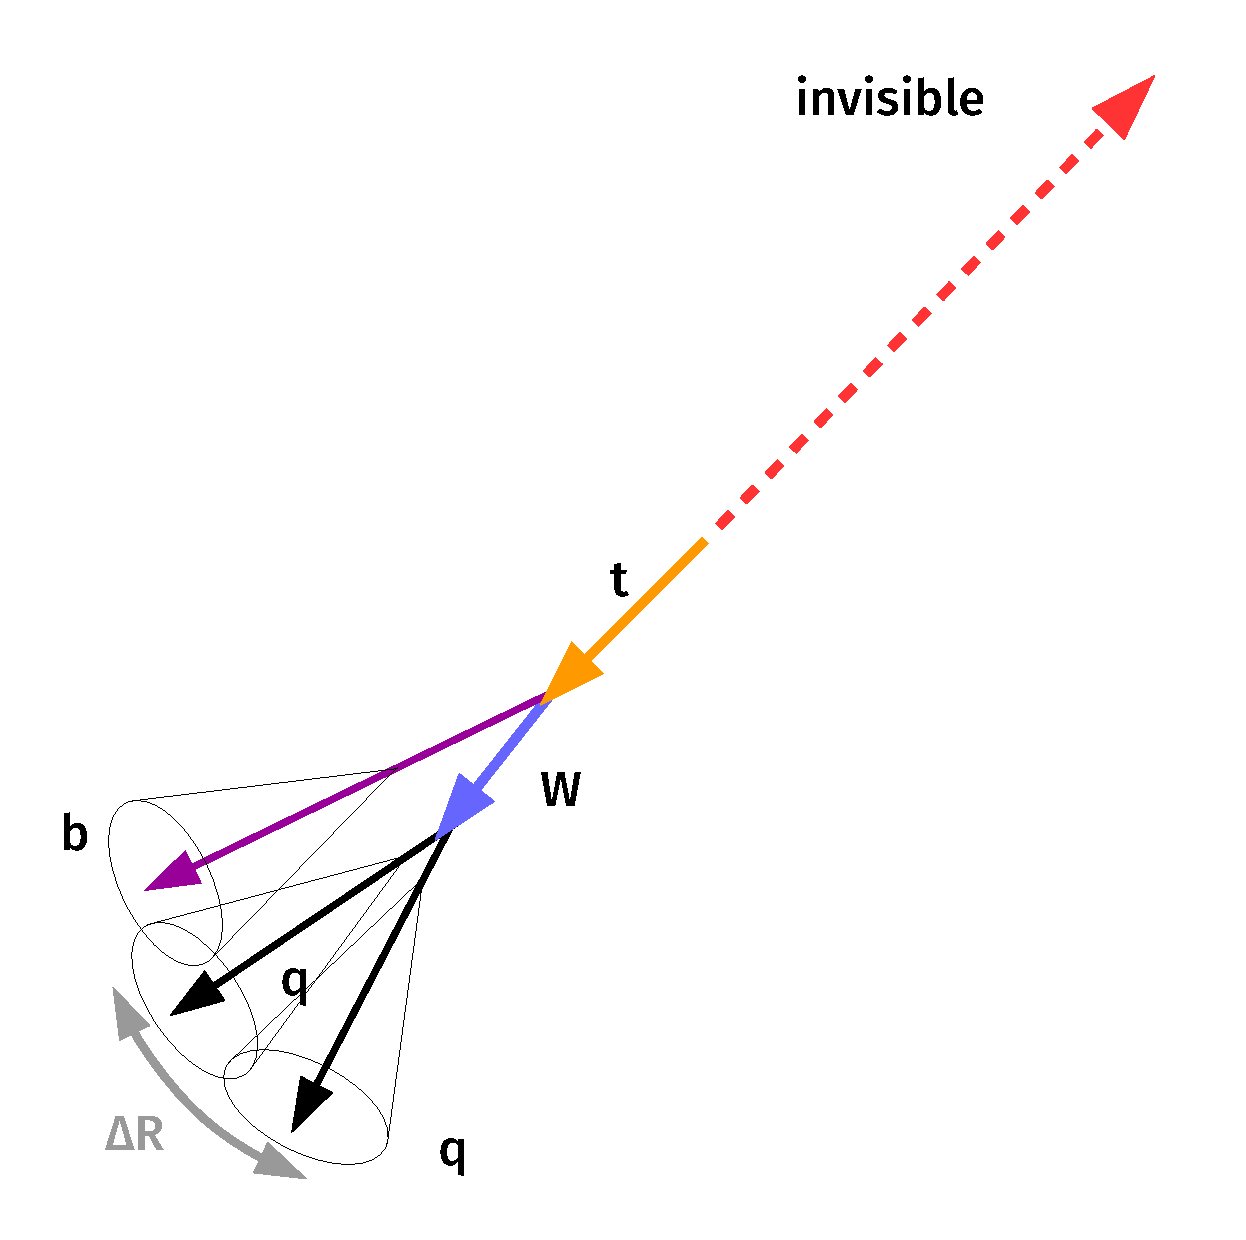
\includegraphics[width=0.8\textwidth]{figs/sketches/boosted_event.pdf}
%   \end{column}
%   \begin{column}{0.5\textwidth}
%     \begin{itemize}
%       \item $\ptmiss>250\,\gev$ (trigger threshold)
%       \item CA15 jet, $\pt>250\,\gev$
%       \begin{itemize}
%         \item Selected by BDT \pause
%         \item Mass consistent with $m_t$
%         \item Signature of $B$ meson decay inside jet
%         \begin{itemize}
%           \item Lab frame $c\tau \sim \mathcal{O} (\mathrm{mm})$
%         \end{itemize}
%       \end{itemize}
%     \end{itemize}
%     \centering
%     \hspace{-30mm}
%       \includegraphics[width=0.45\textwidth]{../../figs/monotop/v14/prefit_unblind/shapes/onefatjet/singlemuontop_fj1MSD.pdf}
%       \includegraphics[width=0.75\textwidth]{figs/SoftDropSubJet_CSVIVFv2_Log.pdf}
%   \end{column}
%   \end{columns}
% \end{frame}
% 
% \begin{frame}[t]  \frametitle{SM backgrounds}
%   \centering
%   \vspace{5mm}
%   \begin{columns}
%   \begin{column}{0.33\textwidth}
%     \centering
%     $Z\rightarrow\nu\nu $ ($30\%$) \\
%     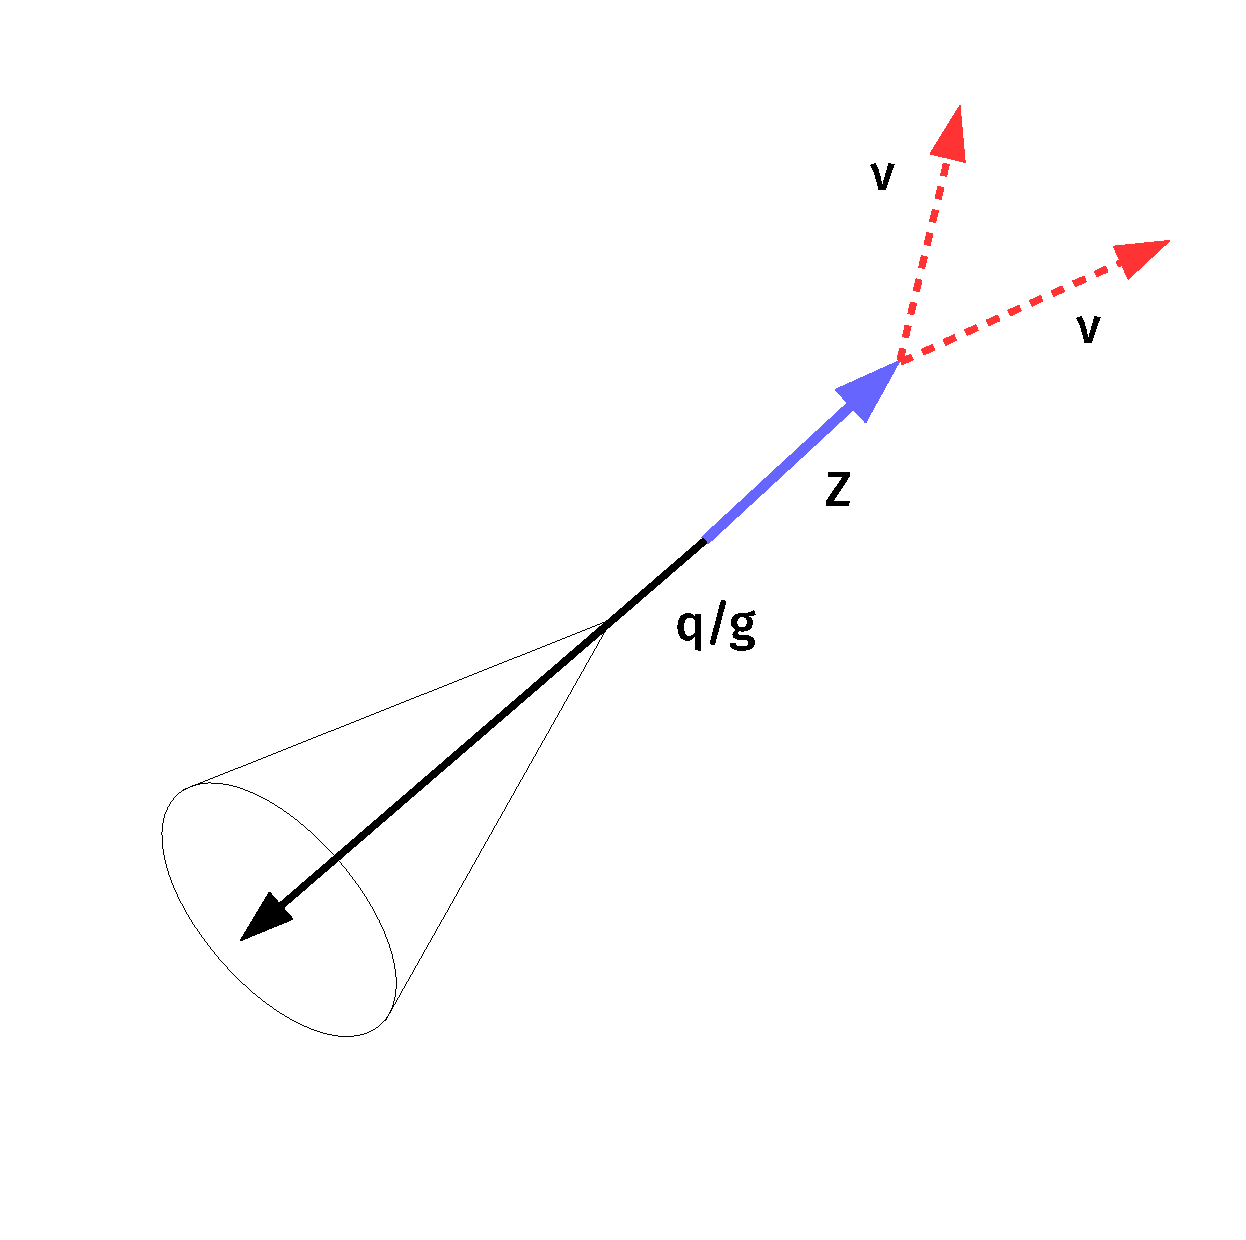
\includegraphics[width=\textwidth]{figs/sketches/zsr.pdf} \pause
%   \end{column}
%   \begin{column}{0.33\textwidth}
%     \centering
%     $W\rightarrow (\ell)\nu$ ($15\%$) \\
%     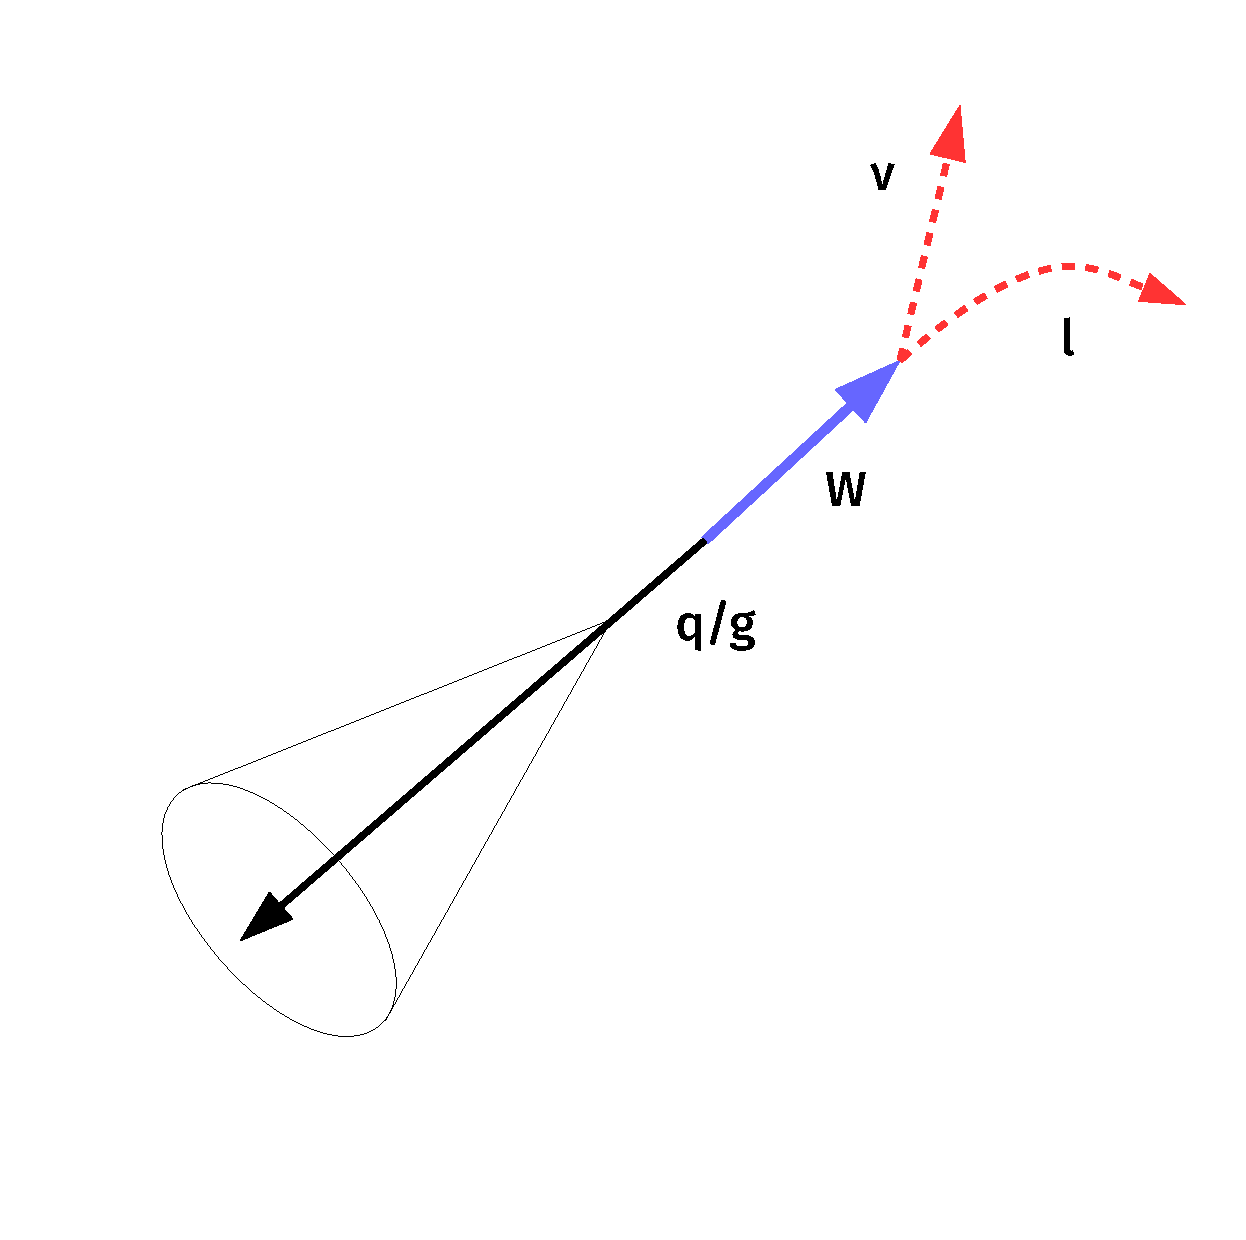
\includegraphics[width=\textwidth]{figs/sketches/wsr.pdf} \pause
%   \end{column}
%   \begin{column}{0.33\textwidth}
%     \centering
%     $t$ quark pair ($50\%$) \\
%     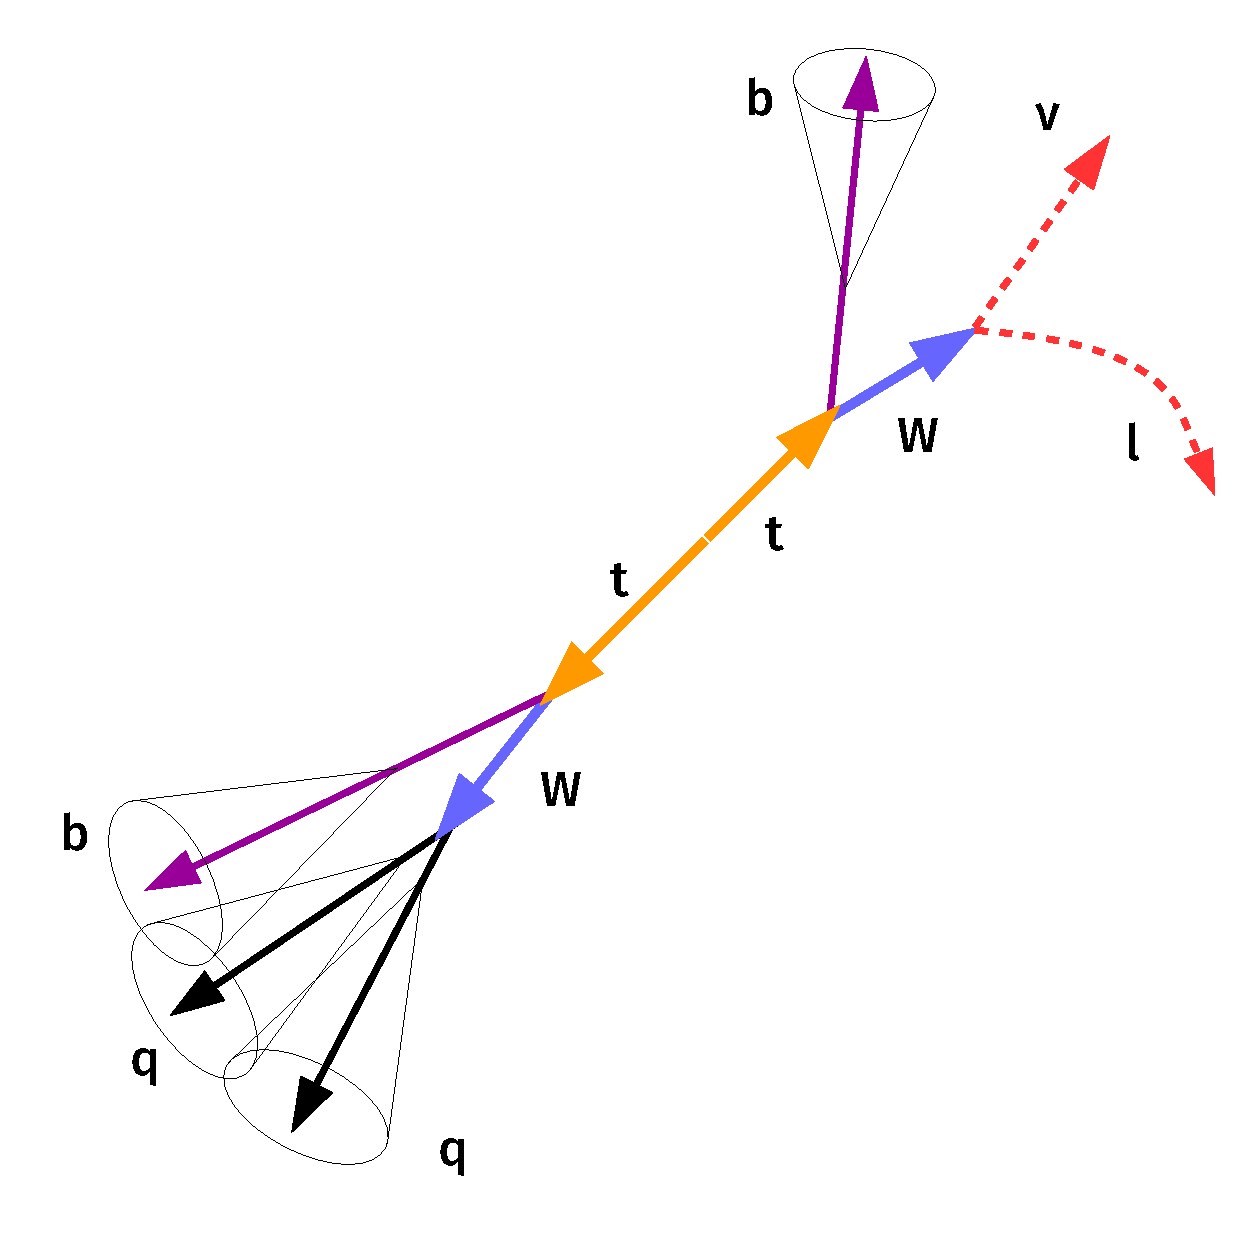
\includegraphics[width=\textwidth]{figs/sketches/ttsr.pdf} \pause
%   \end{column}
%   \end{columns}
%   {\large
%     Note that $\ptmiss$ is the transverse momentum of the \mlink{vector boson}
%   }
% \end{frame}
% 
% \begin{frame}[t]  \frametitle{Background estimation}
%   \begin{columns}
%   \begin{column}{0.33\textwidth}
%     \centering
%     \textcolor{mygrey}{$Z\rightarrow\nu\nu$} \\
%     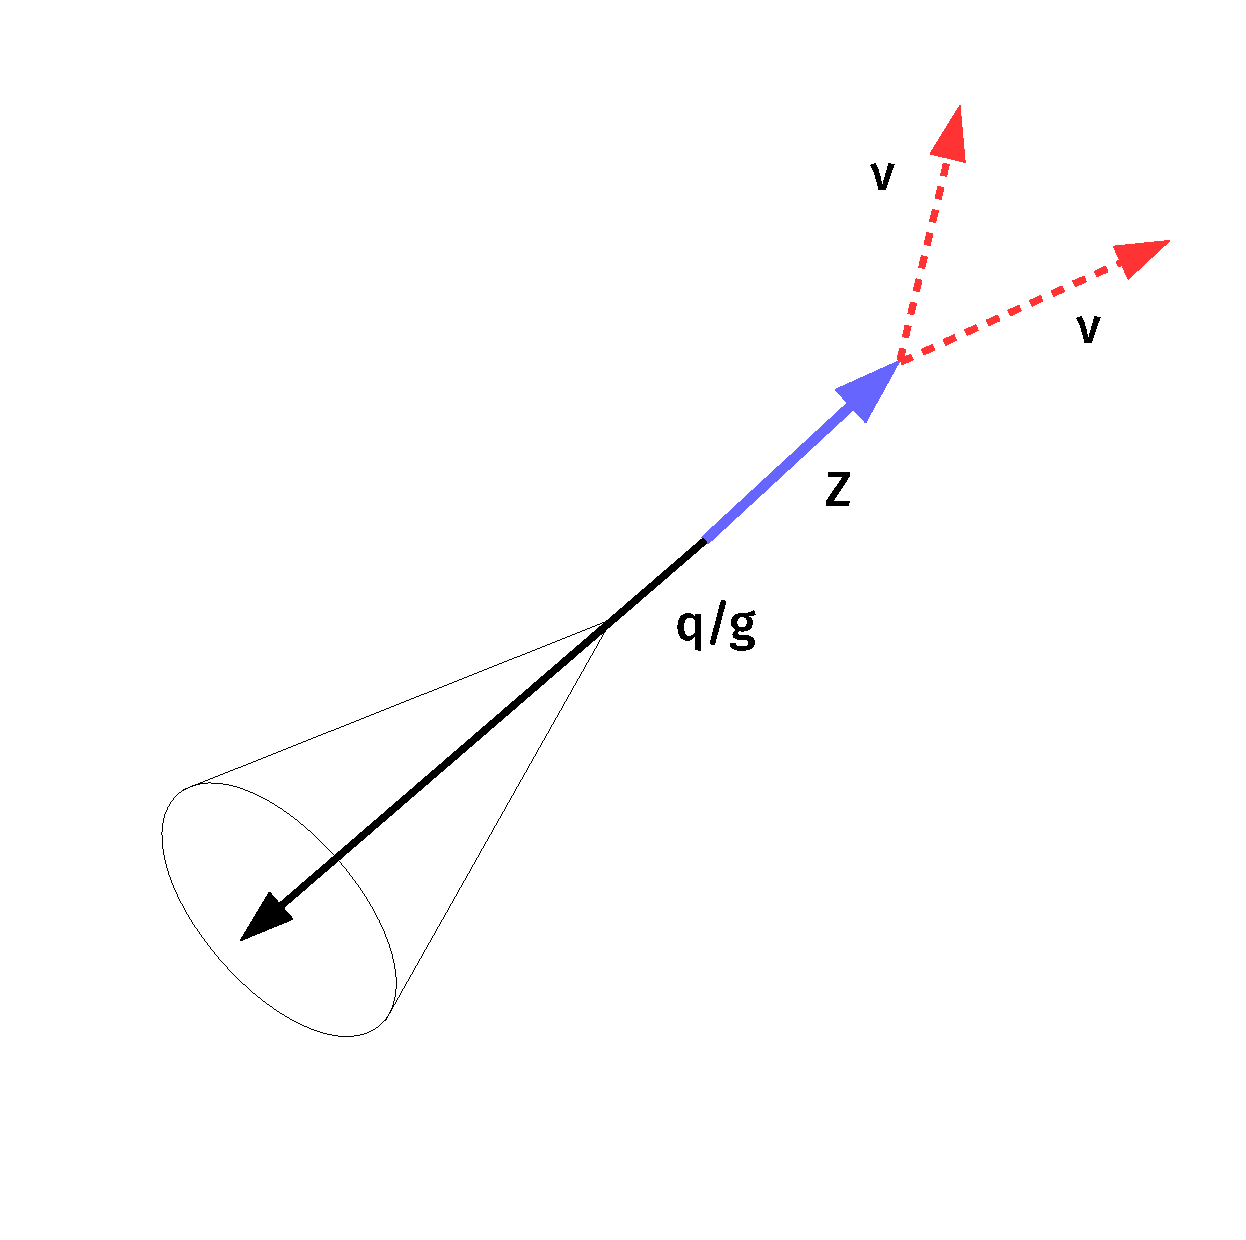
\includegraphics[width=\textwidth]{figs/sketches/zsr.pdf}
%   \end{column}
%   \begin{column}{0.34\textwidth}
%     \centering
%     Ideally: \\
%     {\Large \textcolor{mygrey}{$\ptmiss$}$ \,= \pt^Z =\,$\textcolor{maroon}{$ \pt^{\ell\ell}  $}} \\
%     \vspace{5mm}
%     \uncover<2->{
%     In practice: \\
%     {\Large \textcolor{mygrey}{$\ptmiss$}$ \,\approx \pt^Z \approx\,$\textcolor{maroon}{$ \ptmiss(\mathrm{no}~\ell)$}}
%     }
%   \end{column}
%   \begin{column}{0.33\textwidth}
%     \centering
%     \textcolor{maroon}{$Z\rightarrow\ell\ell$} \\
%     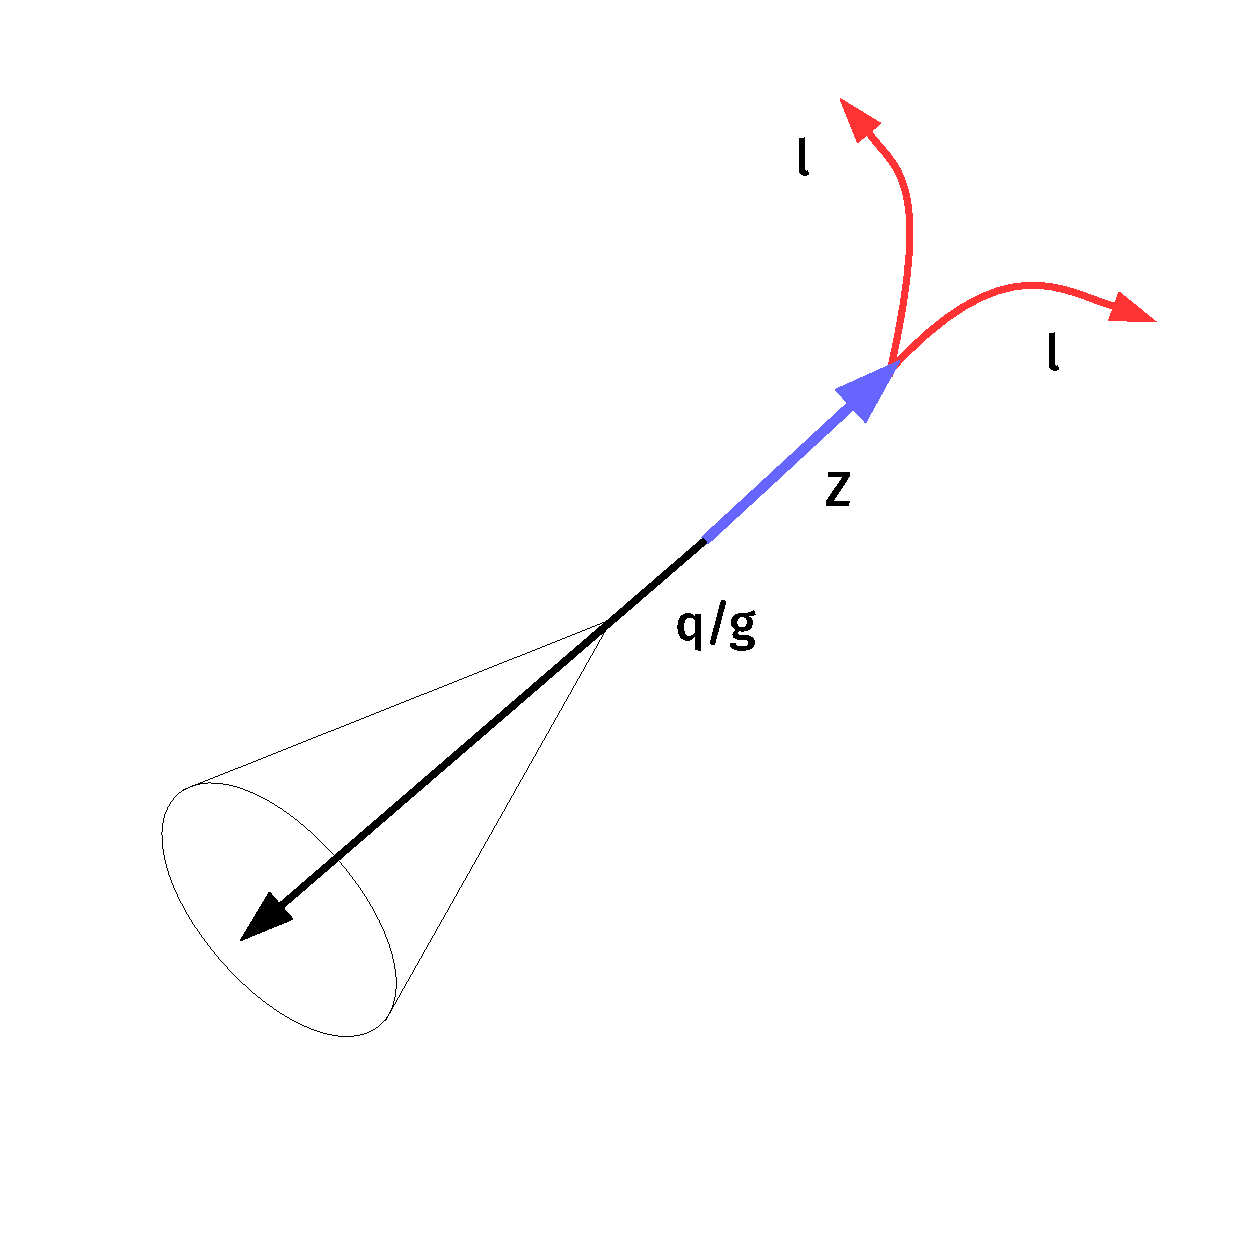
\includegraphics[width=\textwidth]{figs/sketches/zcr.pdf}
%   \end{column}
%   \end{columns}
% 
%   \uncover<2->{
%   \vspace{5mm}
%   \centering
%     \mlink{Hadronic recoil} $\equiv$ momentum imbalance if we pretend $\ell^\pm$ are invisible. \\
%     Only syst.~uncertainty on this extrapolation comes from $\ell$ ID ($\sim1\mathrm{-}3\%$)}
% \end{frame}
% 
% \begin{frame} \frametitle{$\mathcal{B}{(Z\rightarrow\nu\nu)} > \mathcal{B}{(Z\rightarrow\ell\ell)}$}
%   \begin{columns}
%     \begin{column}{0.5\textwidth}
%       \centering
%       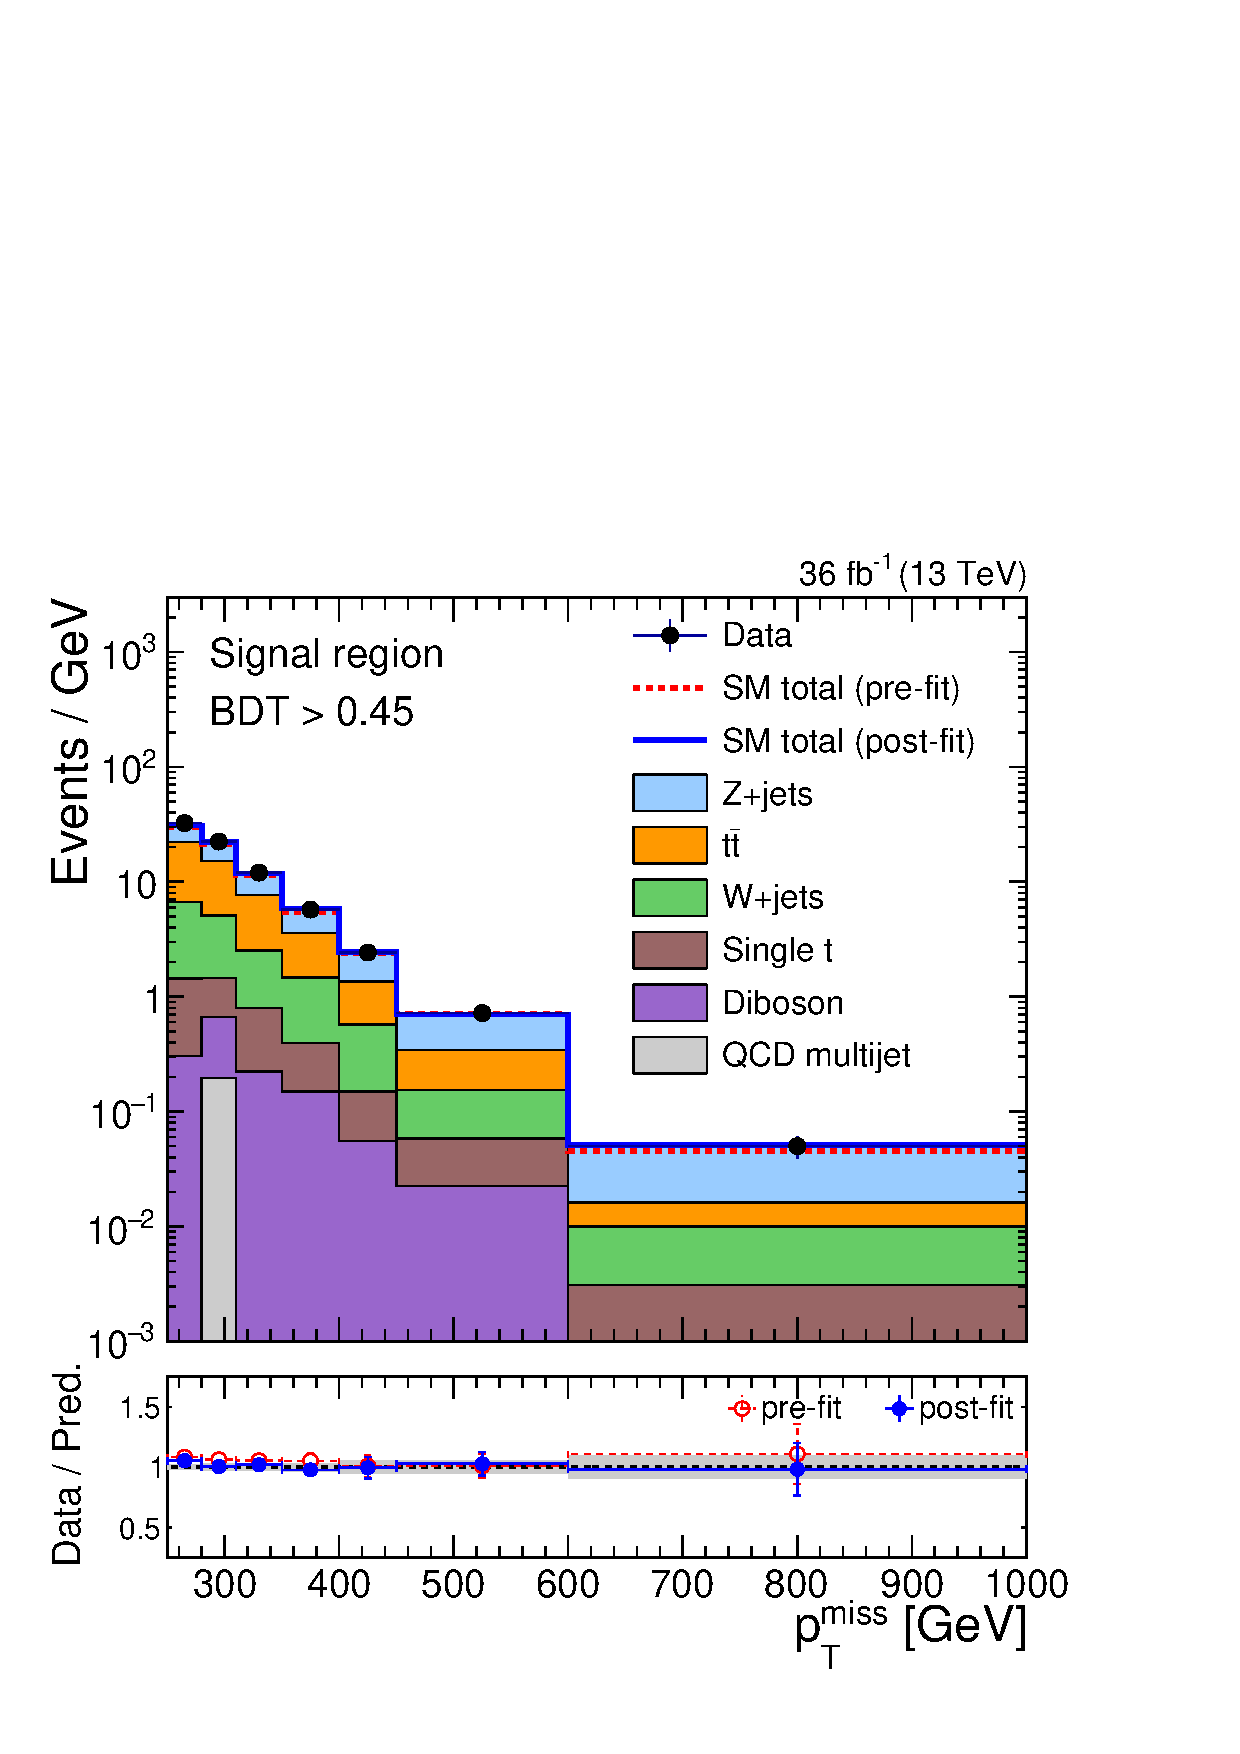
\includegraphics[width=0.8\textwidth]{../../figs/monotop/v14/fr/brown/stackedPostfit_signal_monotop.pdf}
%     \end{column}
%     \begin{column}{0.5\textwidth}
%       \centering
%       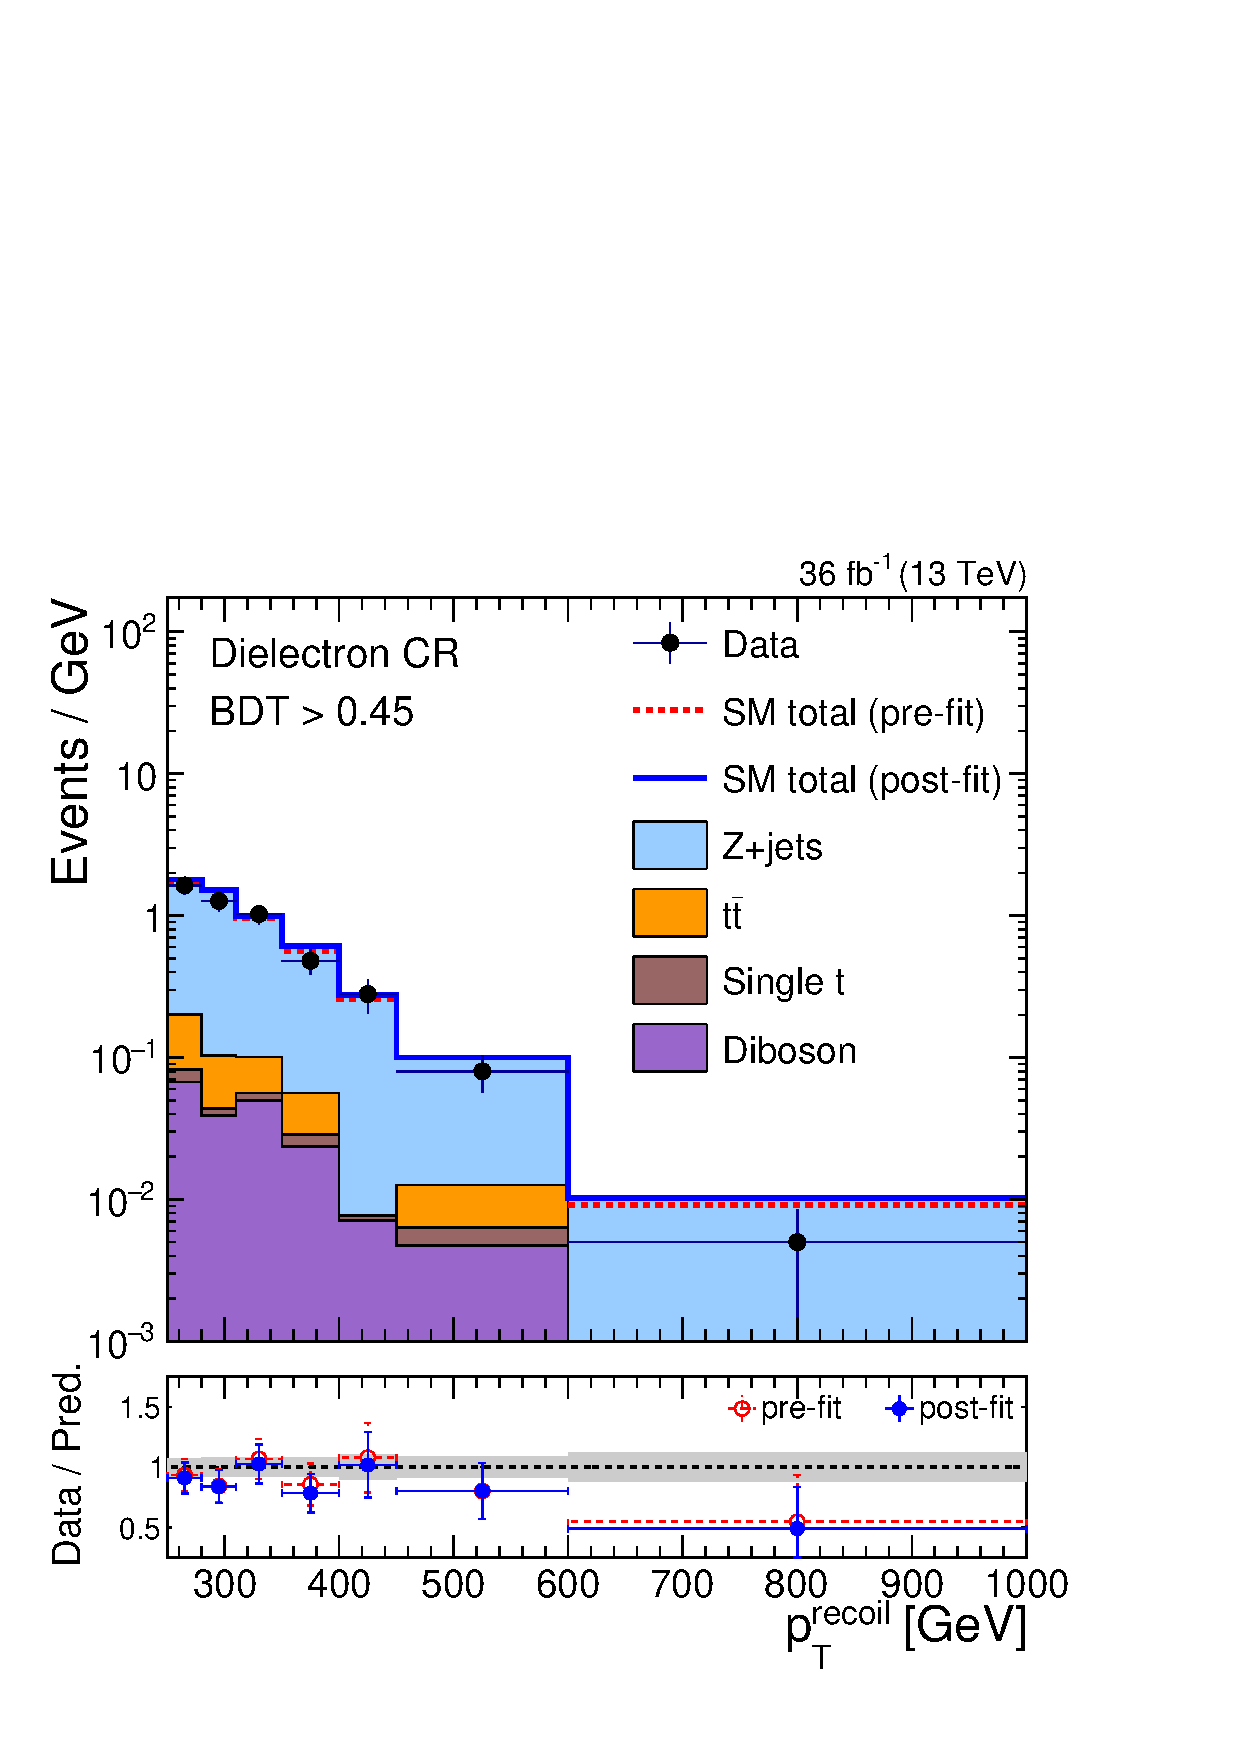
\includegraphics[width=0.8\textwidth]{../../figs/monotop/v14/fr/brown/stackedPostfit_dielectron_monotop.pdf}
%     \end{column}
%   \end{columns}
% \end{frame}
% 
% \begin{frame} \frametitle{$\sigma(\gamma) \gg \sigma(W) > \sigma{(Z)}$}
%   \centering
%       Use production of $\gamma$ and $W$ to estimate production of $Z$
%   \begin{columns}
%     \begin{column}{0.5\textwidth}
%       \centering
%       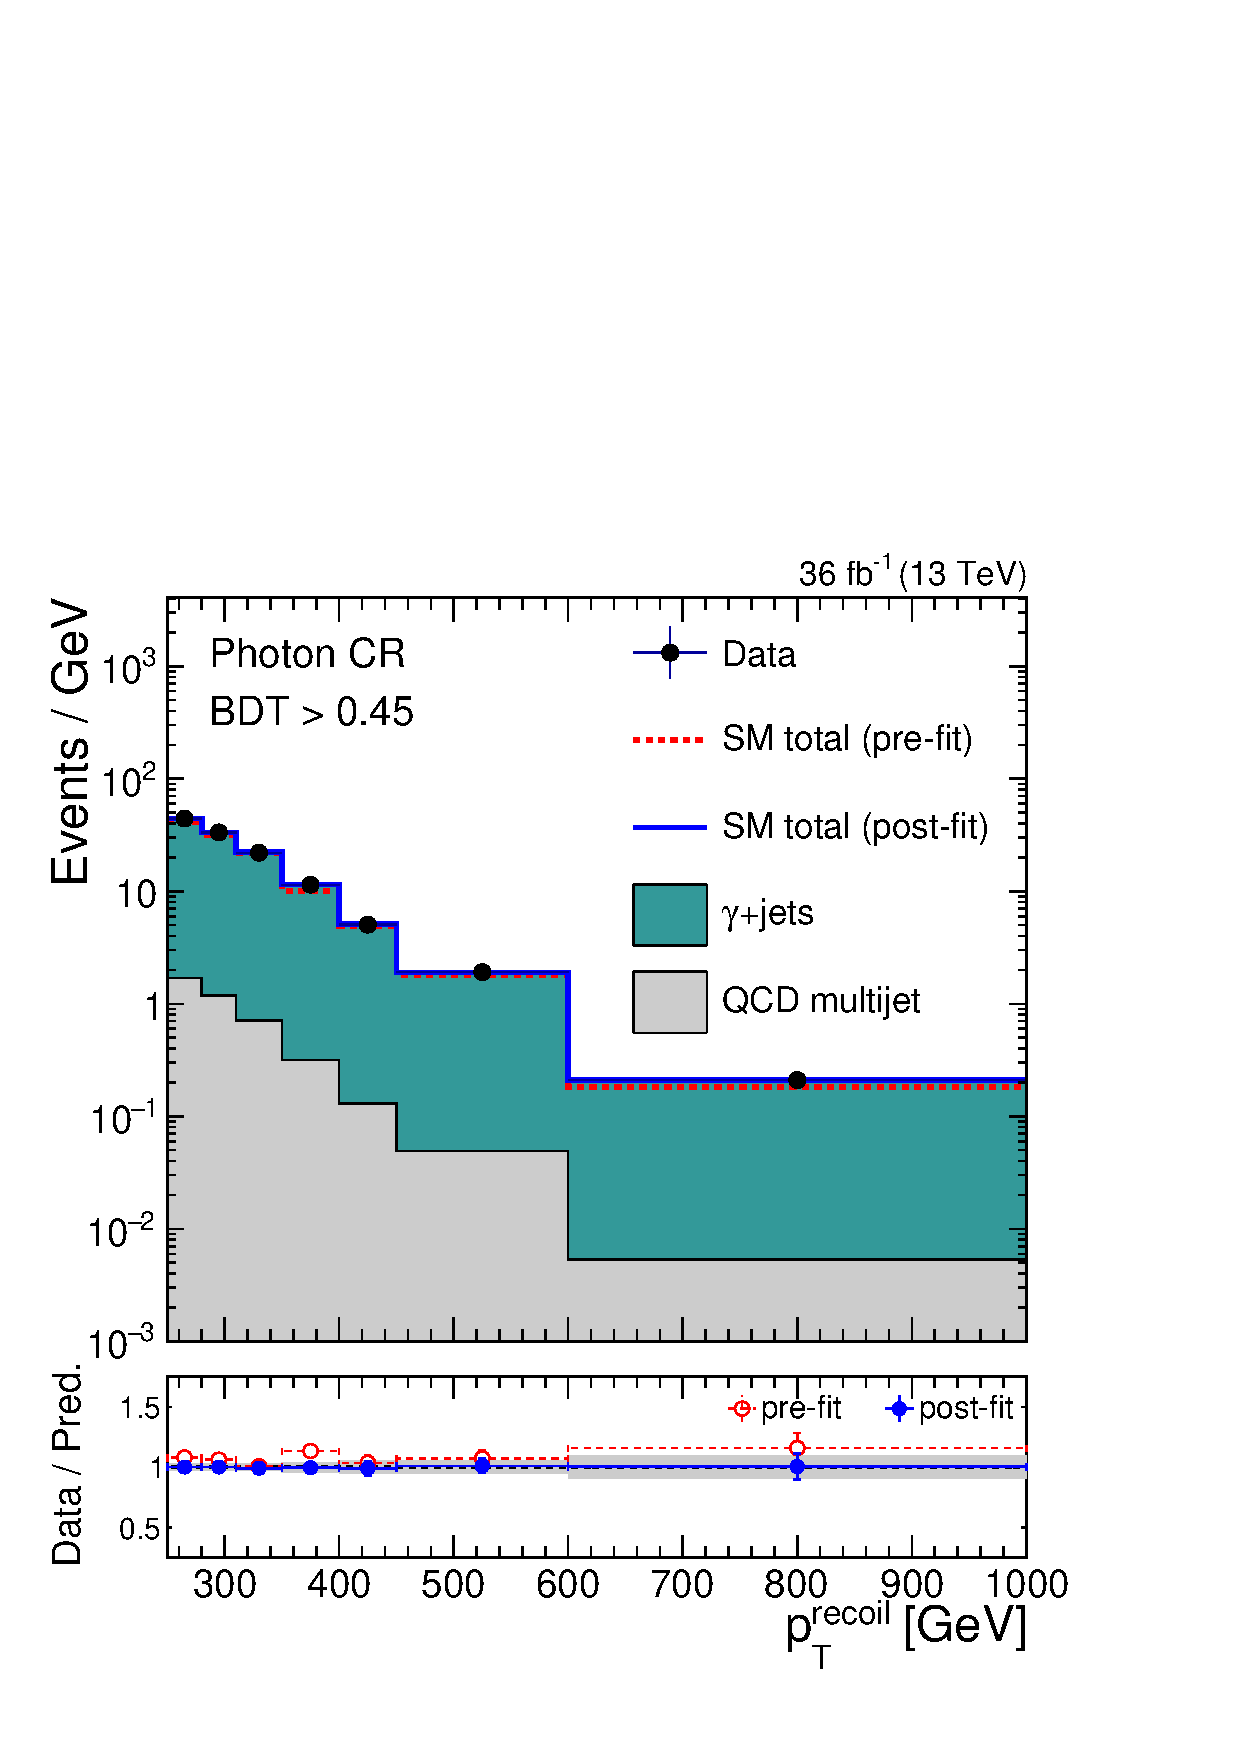
\includegraphics[width=0.8\textwidth]{../../figs/monotop/v14/fr/brown/stackedPostfit_photon_monotop.pdf}
%     \end{column}
%     \begin{column}{0.5\textwidth}
%       \centering
%       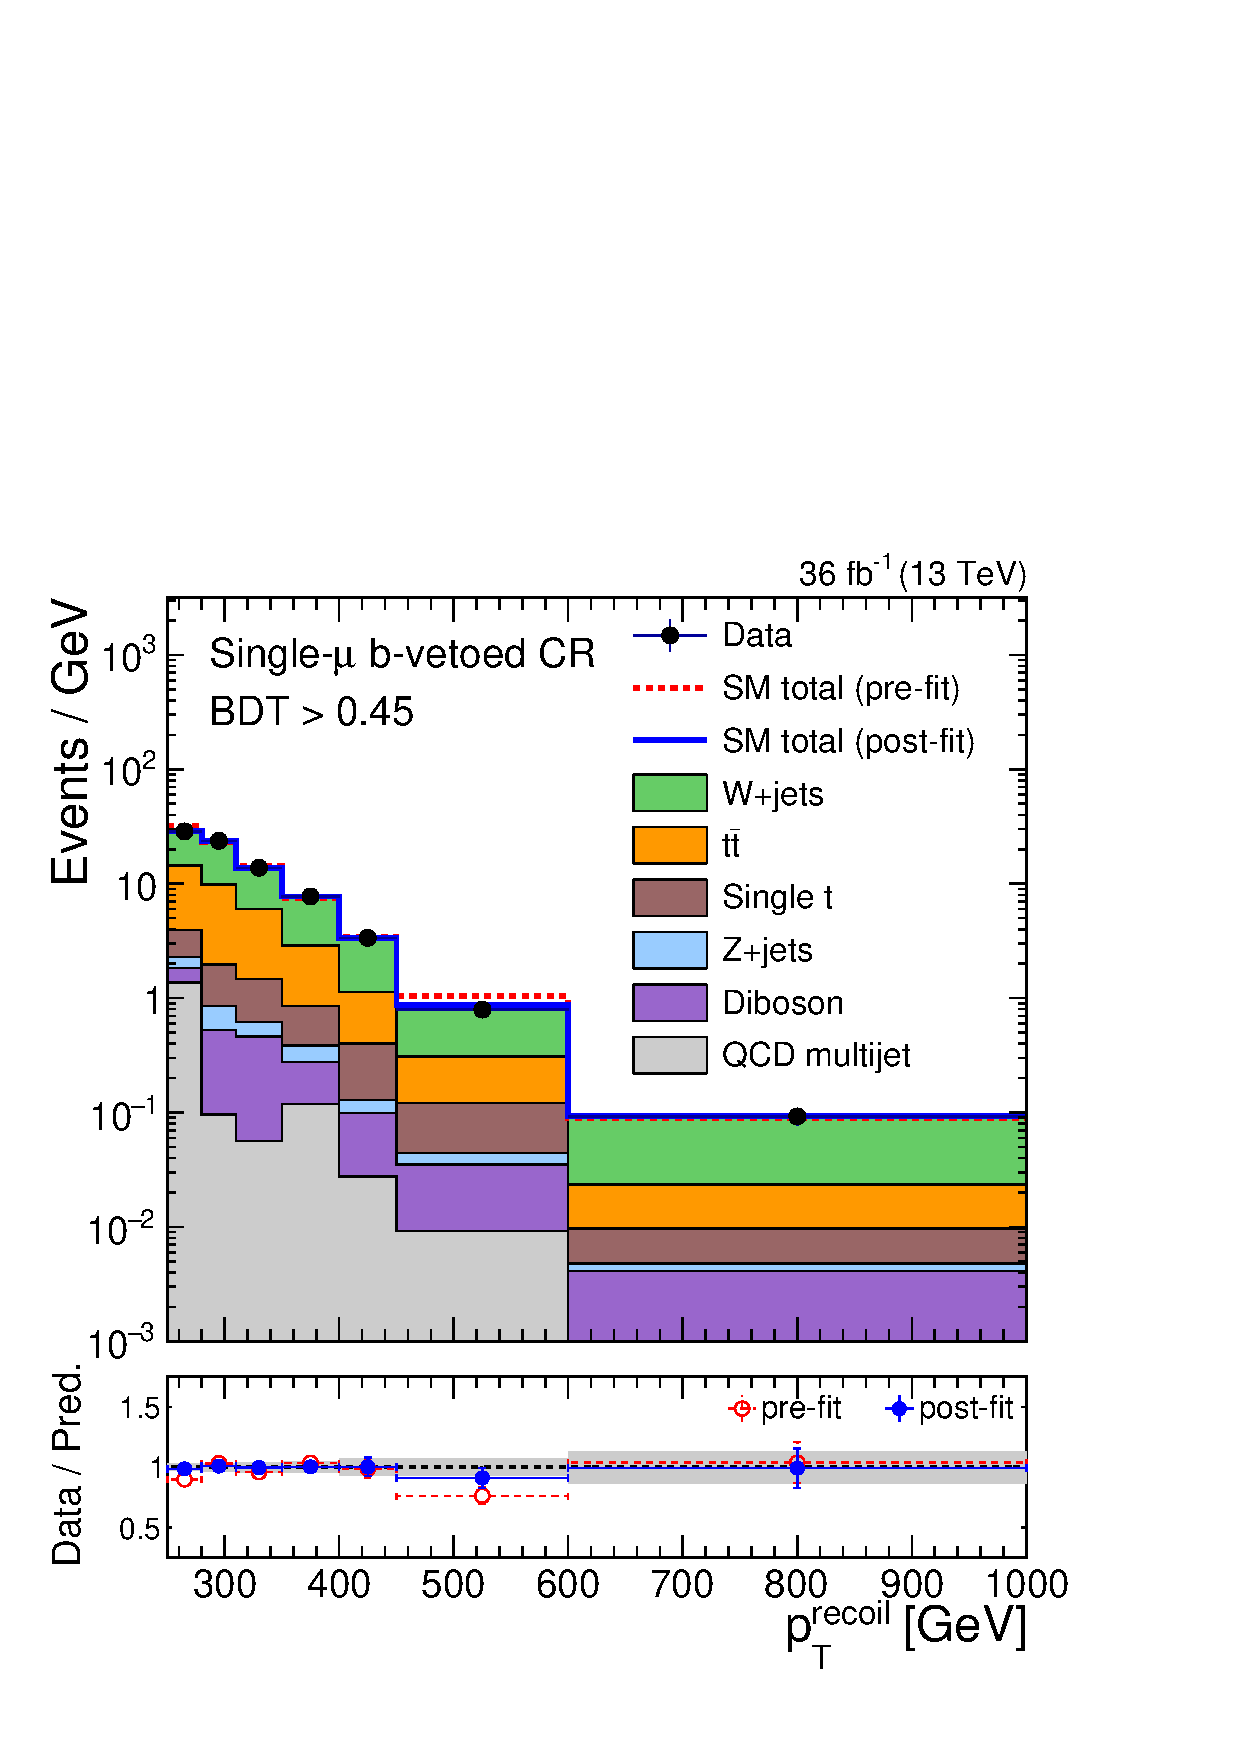
\includegraphics[width=0.8\textwidth]{../../figs/monotop/v14/fr/brown/stackedPostfit_singlemuonw_monotop.pdf}
%     \end{column}
%   \end{columns}
% \end{frame}
% 
% \begin{frame} \frametitle{Fitting ratios}
%   \vspace{-5mm}
%   \begin{itemize}
%     \item Free parameters in fit are:
%     \[\bmu_i^{Z\rightarrow\nu\nu}\text{ - number of $Z$ events in SR}\]
%     \[\bR_i^{X}(\bm{\theta})\text{ - ratio of events in SR and CR $X$}\]
%     \item Each extrapolation $\Rightarrow$ an additional $\bR$
%     {\small
%     \begin{align*}
%   \mathcal{L}(\bmu^{Z\rightarrow\nu\nu};\pmb\theta) ~=
%     & \prod_{i\in\text{bins}} \text{Poisson} \left(d_i^\text{signal}\Big| B_i^\text{signal}(\pmb\theta)
%                                                            + (1+f_i(\pmb\theta))\bmu^{Z\rightarrow\nu\nu}_i
%                                                            + \mu S_i(\pmb\theta) \right) \\
%     & \times \prod_{i\in\text{bins}} \text{Poisson} \left(d_i^{\ell\ell}\Big| B_i^{\ell\ell}(\pmb\theta)
%                                                    + \frac{\bmu^{Z\rightarrow\nu\nu}_i}{\bR^{\ell\ell}_i(\pmb\theta)} \right) \nonumber \\
%     & \times \cdots
%     \end{align*}
%                                                          }
%     \item Physics challenge boils down to predicting and assigning uncertainty on $\bR$
%   \end{itemize}
% \end{frame}
% 
% \begin{frame} \frametitle{Extrapolation uncertainties}
%   \vspace{-5mm}
%   \begin{columns}
%     \begin{column}{0.5\textwidth}
%       \centering
%       $t\bar{t}\rightarrow b\mu\nu+$jets \\
%       \only<1>{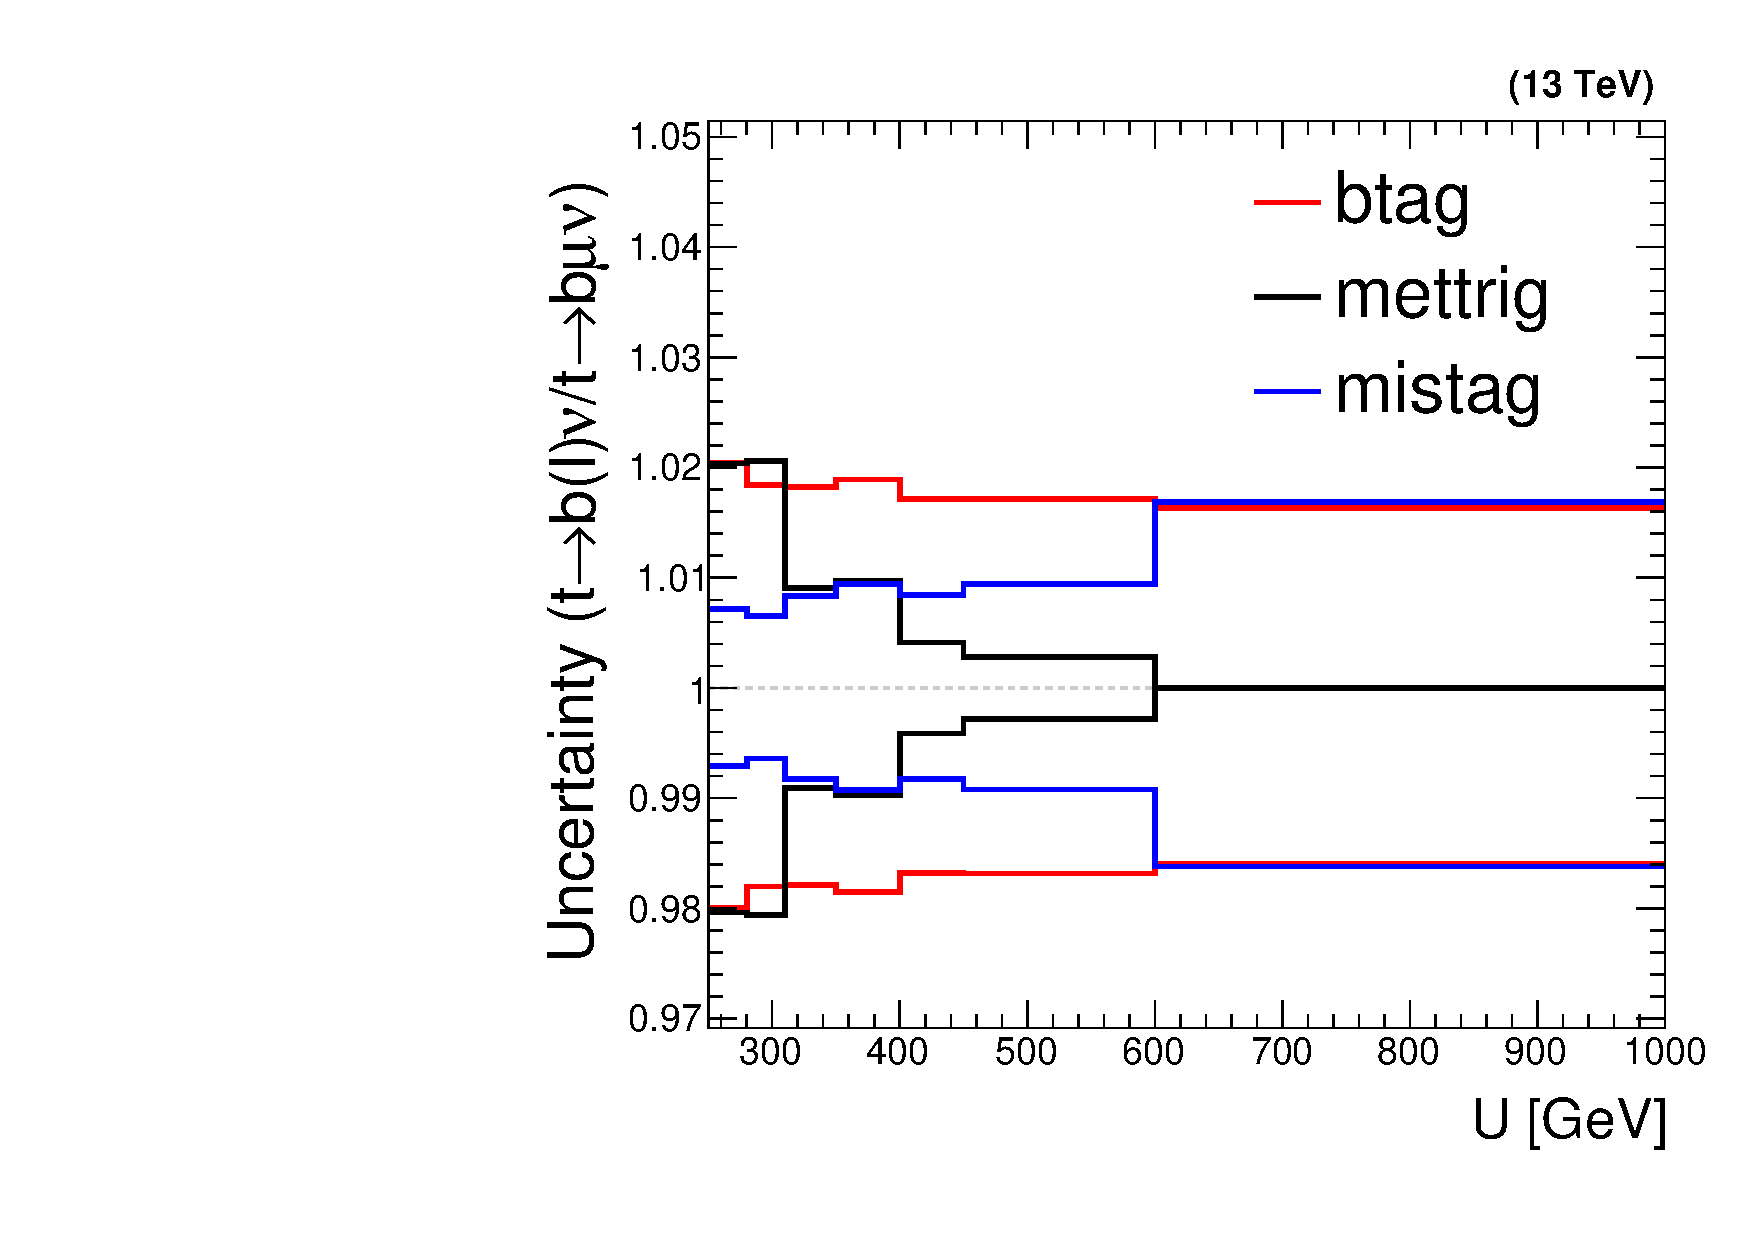
\includegraphics[width=0.8\textwidth]{figs/monotop/fits_unblinded/variations_singlemuontop.pdf}} \\
%       Small experimental uncertainties
%     \end{column}
%     \begin{column}{0.5\textwidth}
%       \centering
%       $W\rightarrow\ell\nu $ \\
%       \only<1>{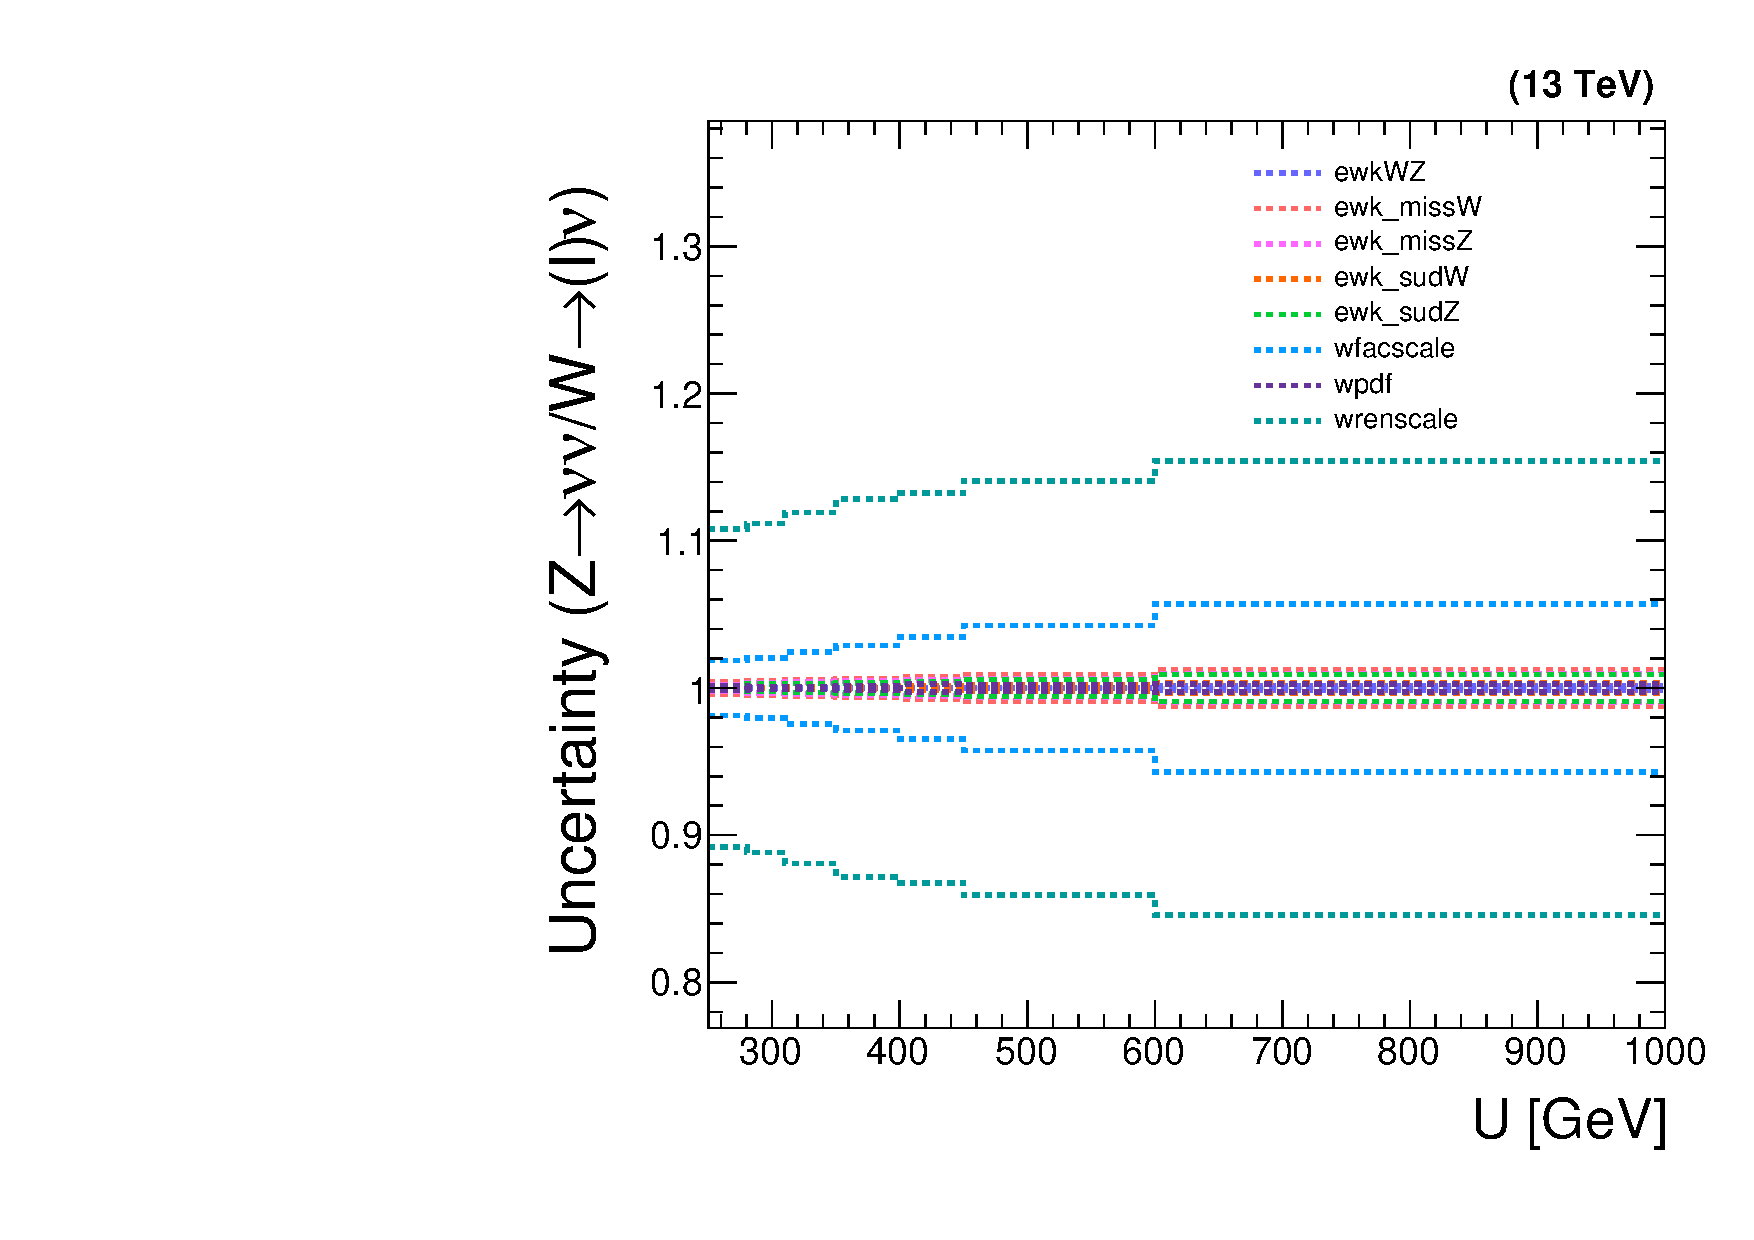
\includegraphics[width=0.8\textwidth]{figs/monotop/fits_unblinded/variations_wz.pdf}} \\
%       Large theoretical uncertainties
%     \end{column}
%   \end{columns}
% \end{frame}
% 
% \begin{frame}[t]  \frametitle{Background estimation summary}
%   \begin{minipage}{\textwidth}
%   \centering
%   \begin{tikzpicture}[<->,>=stealth',shorten >=1pt,auto,node distance=3cm,
%                     semithick,text width=1.5cm,align=center]
%     % \tikzstyle{every state}=[fill=red,draw=none,text=white]
% 
%     \node[state,color=red] (ZvvSR)                    {\textcolor{black}{$Z\rightarrow\nu\nu$\\SR}};
%     \node[state,color=blue] (ZllCR) [above left of=ZvvSR] {\textcolor{black}{$Z\rightarrow\ell\ell$\\ $\ell\ell$ CR}};
%     \node(ZllDiag) [right of=ZllCR] {\hspace{-12mm}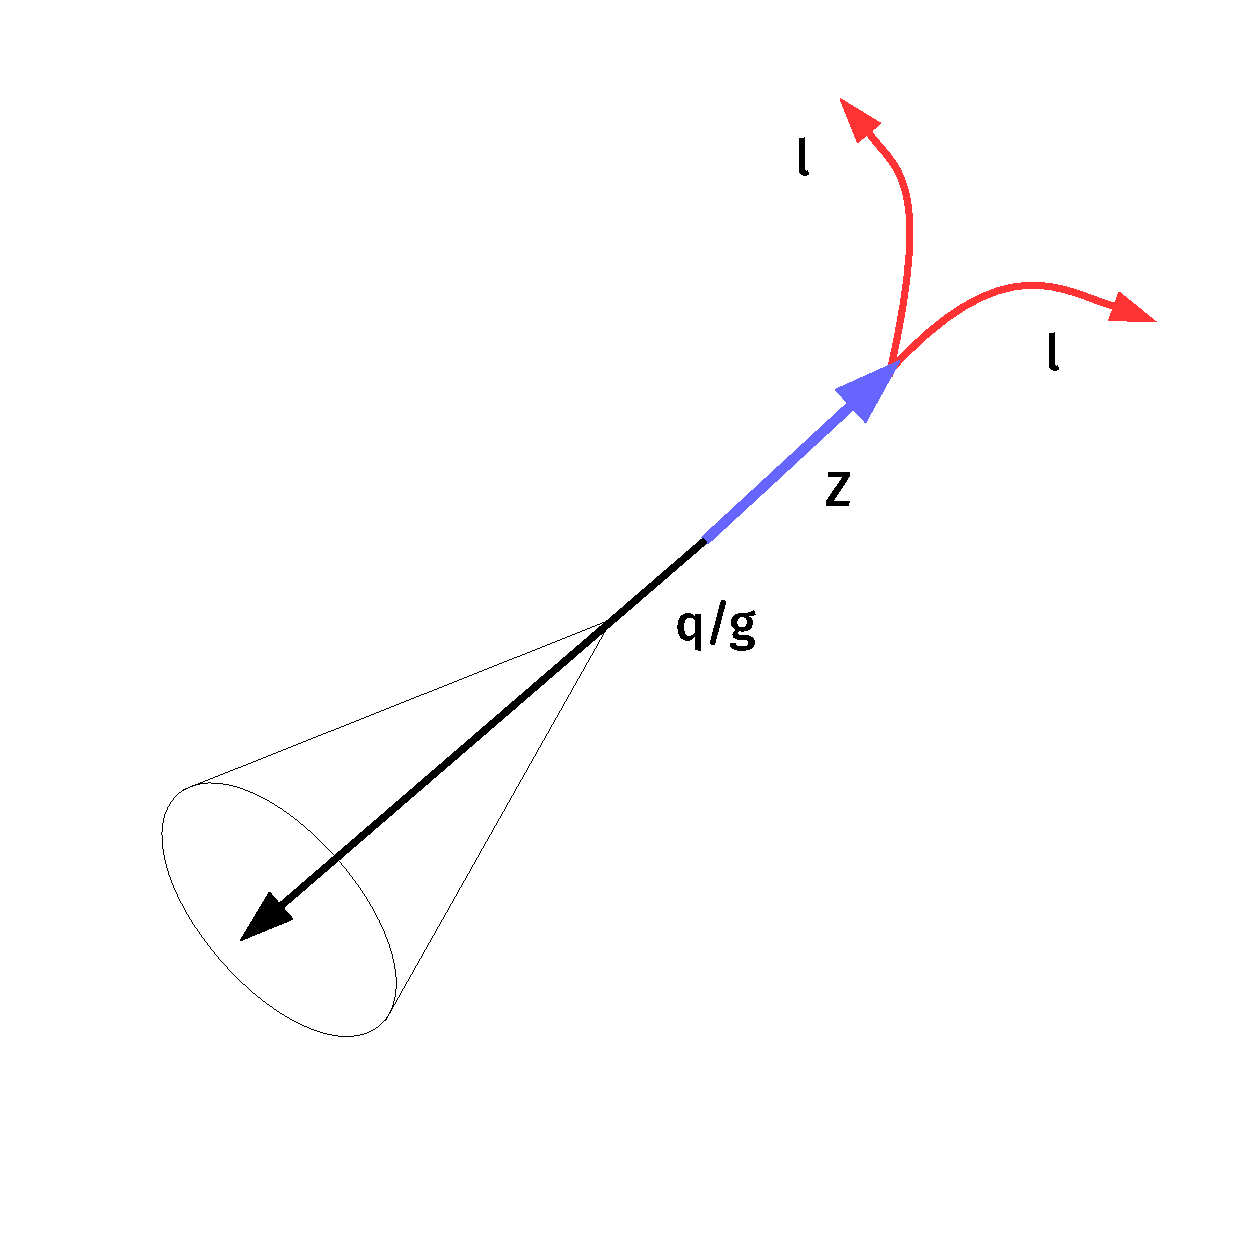
\includegraphics[width=1.5\textwidth]{figs/sketches/zcr.pdf}};
% 
%     \path[dashed]
%           (ZvvSR) edge          node {} (ZllCR)
%     ;
%   \end{tikzpicture}
%   \end{minipage}
% \end{frame}
% 
% \begin{frame}[t]   \frametitle{Background estimation summary}
%   \begin{minipage}{\textwidth}
%   \centering
%   \begin{tikzpicture}[<->,>=stealth',shorten >=1pt,auto,node distance=3cm,
%                     semithick,text width=1.5cm,align=center]
%     % \tikzstyle{every state}=[fill=red,draw=none,text=white]
% 
%     \node[state,color=red] (ZvvSR)                    {\textcolor{black}{$Z\rightarrow\nu\nu$\\SR}};
%     \node[state,color=blue] (ZllCR) [above left of=ZvvSR] {\textcolor{black}{$Z\rightarrow\ell\ell$\\ $\ell\ell$ CR}};
%     \node[state,color=black!60!blue] (ACR) [below left of=ZvvSR] {\textcolor{black}{$\gamma$\\$\gamma$ CR}};
%     \node[state,color=red]         (WlvSR) [right of=ZvvSR]   {\textcolor{black}{$W\rightarrow\ell\nu$\\SR}};
%     \node(ZllDiag) [right of=ZllCR] {\hspace{-12mm}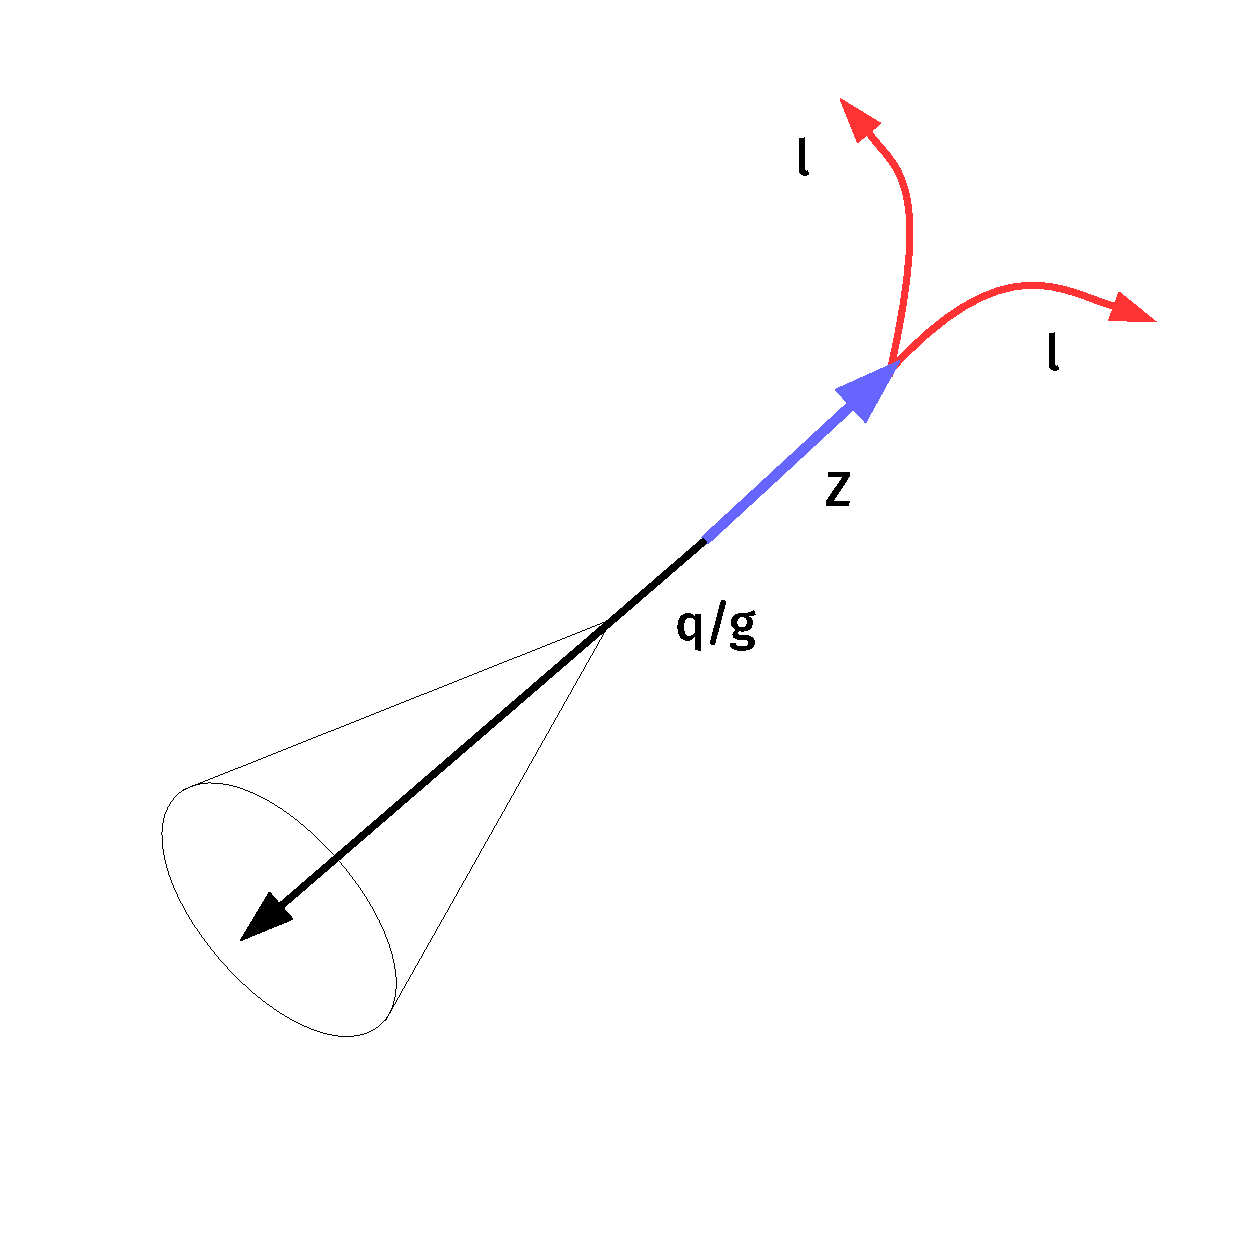
\includegraphics[width=1.5\textwidth]{figs/sketches/zcr.pdf}};
%     \node(ADiag) [right of=ACR] {\hspace{-12mm}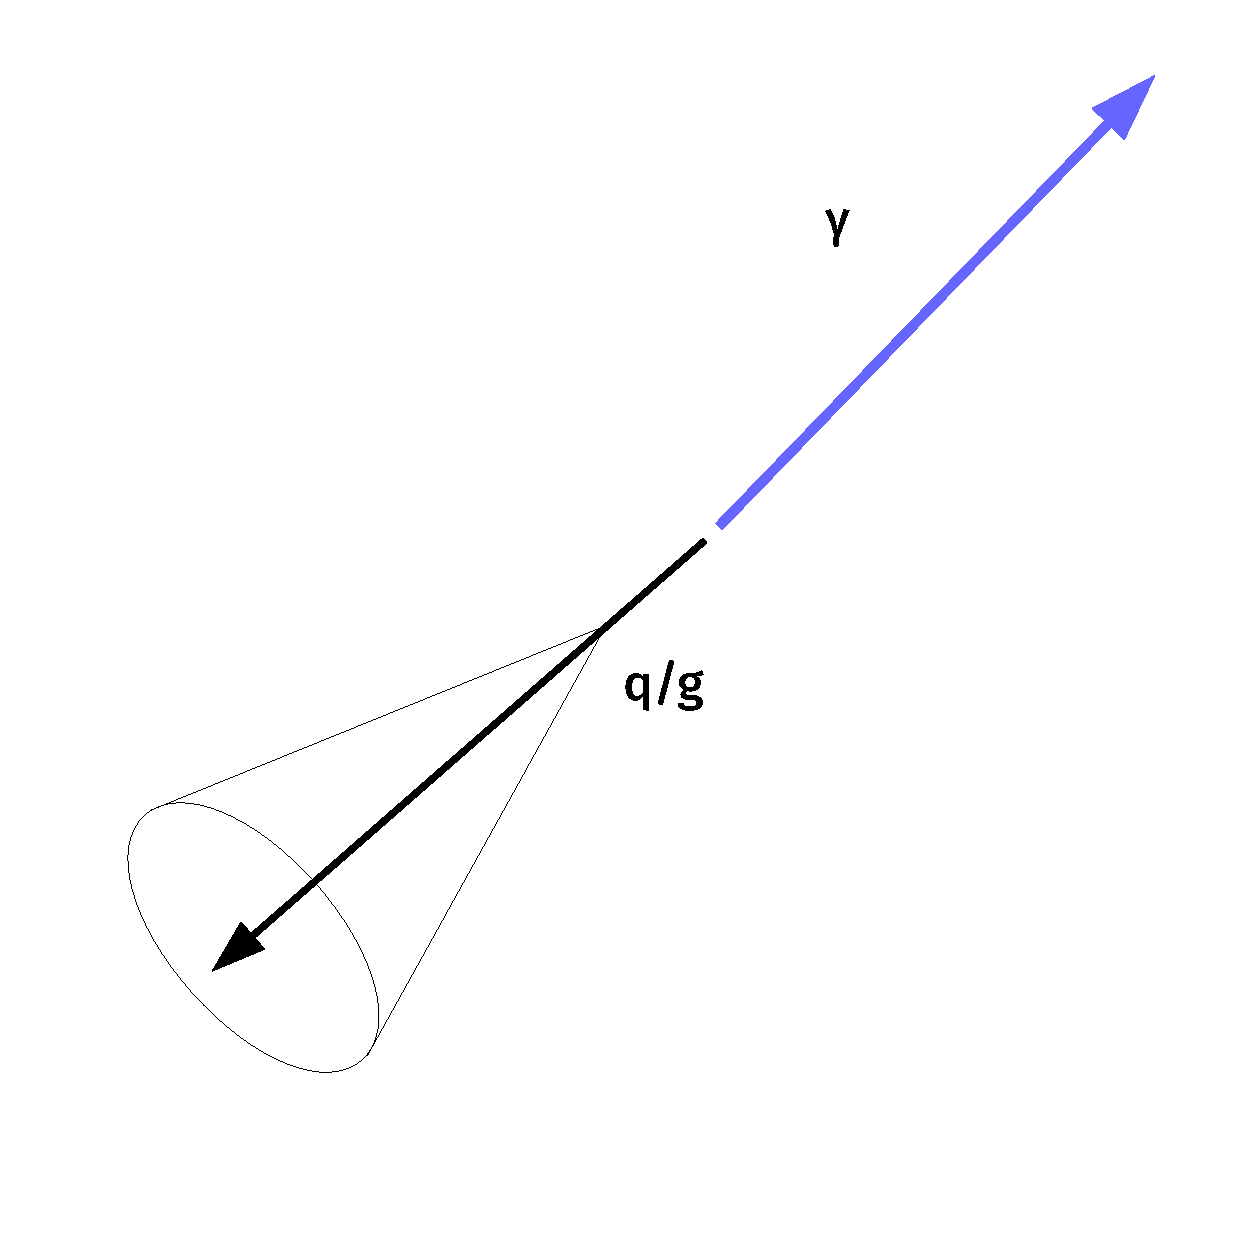
\includegraphics[width=1.5\textwidth]{figs/sketches/acr.pdf}};
% 
%     \path[dashed]
%           (ZvvSR) edge          node {} (ZllCR)
%     ;
%     \path
%           (ZvvSR) edge          node {} (ACR)
%           (ZvvSR) edge          node {} (WlvSR)
%     ;
%   \end{tikzpicture}
%   \end{minipage}
% \end{frame}
% 
% \begin{frame}[t]   \frametitle{Background estimation summary}
%   \begin{minipage}{\textwidth}
%   \centering
%   \begin{tikzpicture}[<->,>=stealth',shorten >=1pt,auto,node distance=3cm,
%                     semithick,text width=1.5cm,align=center]
%     % \tikzstyle{every state}=[fill=red,draw=none,text=white]
% 
%     \node[state,color=red] (ZvvSR)                    {\textcolor{black}{$Z\rightarrow\nu\nu$\\SR}};
%     \node[state,color=blue] (ZllCR) [above left of=ZvvSR] {\textcolor{black}{$Z\rightarrow\ell\ell$\\ $\ell\ell$ CR}};
%     \node[state,color=black!60!blue] (ACR) [below left of=ZvvSR] {\textcolor{black}{$\gamma$\\$\gamma$ CR}};
%     \node[state,color=red]         (WlvSR) [right of=ZvvSR]   {\textcolor{black}{$W\rightarrow\ell\nu$\\SR}};
%     \node[state,color=orange] (WlvCR) [above right of=WlvSR]  {\textcolor{black}{$W\rightarrow\ell\nu$\\$\ell$ CR}};
%     \node[state,color=red] (ttSR) [below right of=WlvCR] {\textcolor{black}{$t\bar{t}$\\SR}};
%     \node[state,color=orange] (ttWCR) [above right of=ttSR]  {\textcolor{black}{$t\bar{t}$\\$\ell$ CR}};
%     \node[state,color=black!60!green] (tttCR) [below right of=ttSR]  {\textcolor{black}{$t\bar{t}$\\$b\ell$ CR}};
%     \node(ZllDiag) [right of=ZllCR] {\hspace{-12mm}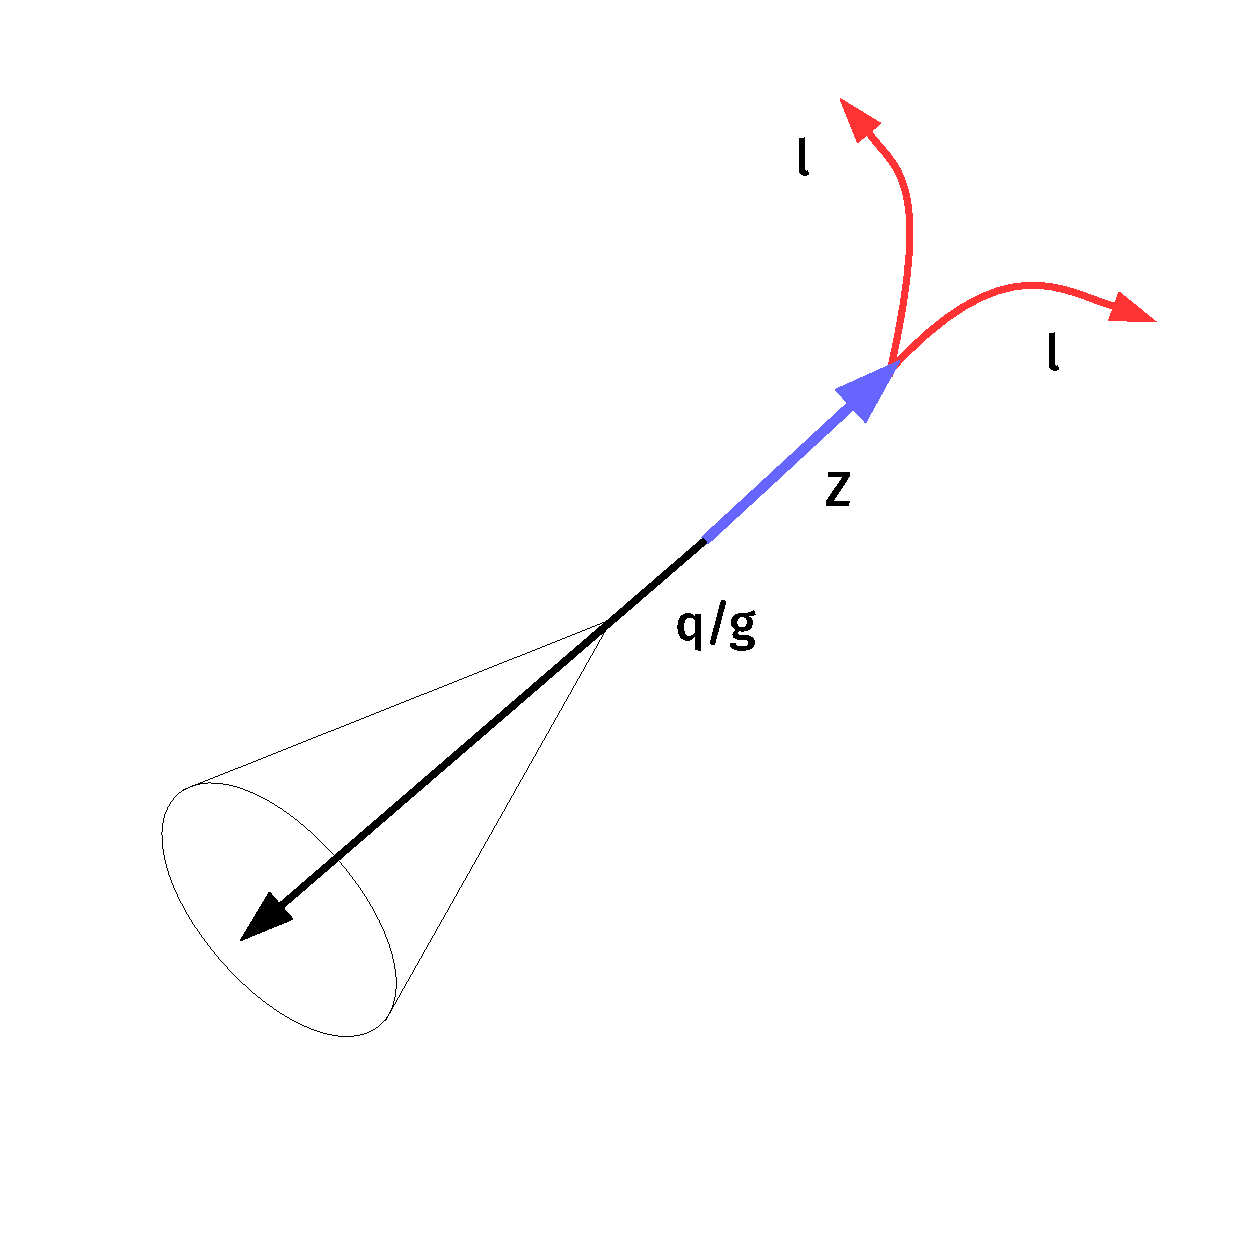
\includegraphics[width=1.5\textwidth]{figs/sketches/zcr.pdf}};
%     \node(WlvDiag) [left of=WlvCR] {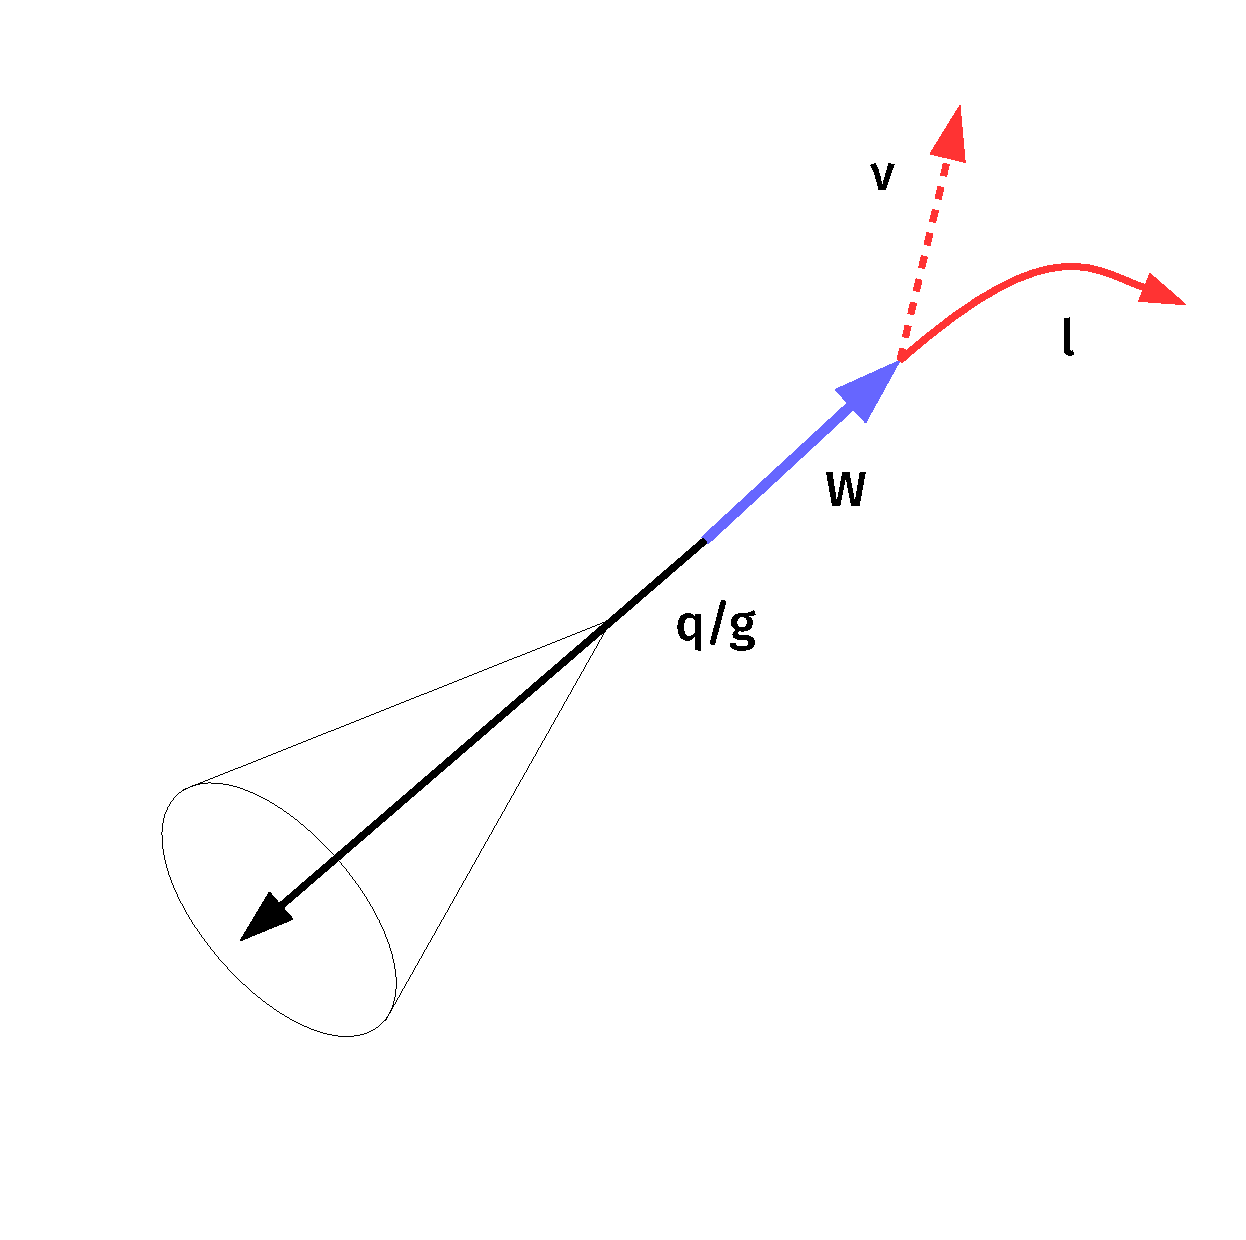
\includegraphics[width=1.5\textwidth]{figs/sketches/wcr.pdf}\hspace{-40mm}};
%     \node(ADiag) [right of=ACR] {\hspace{-12mm}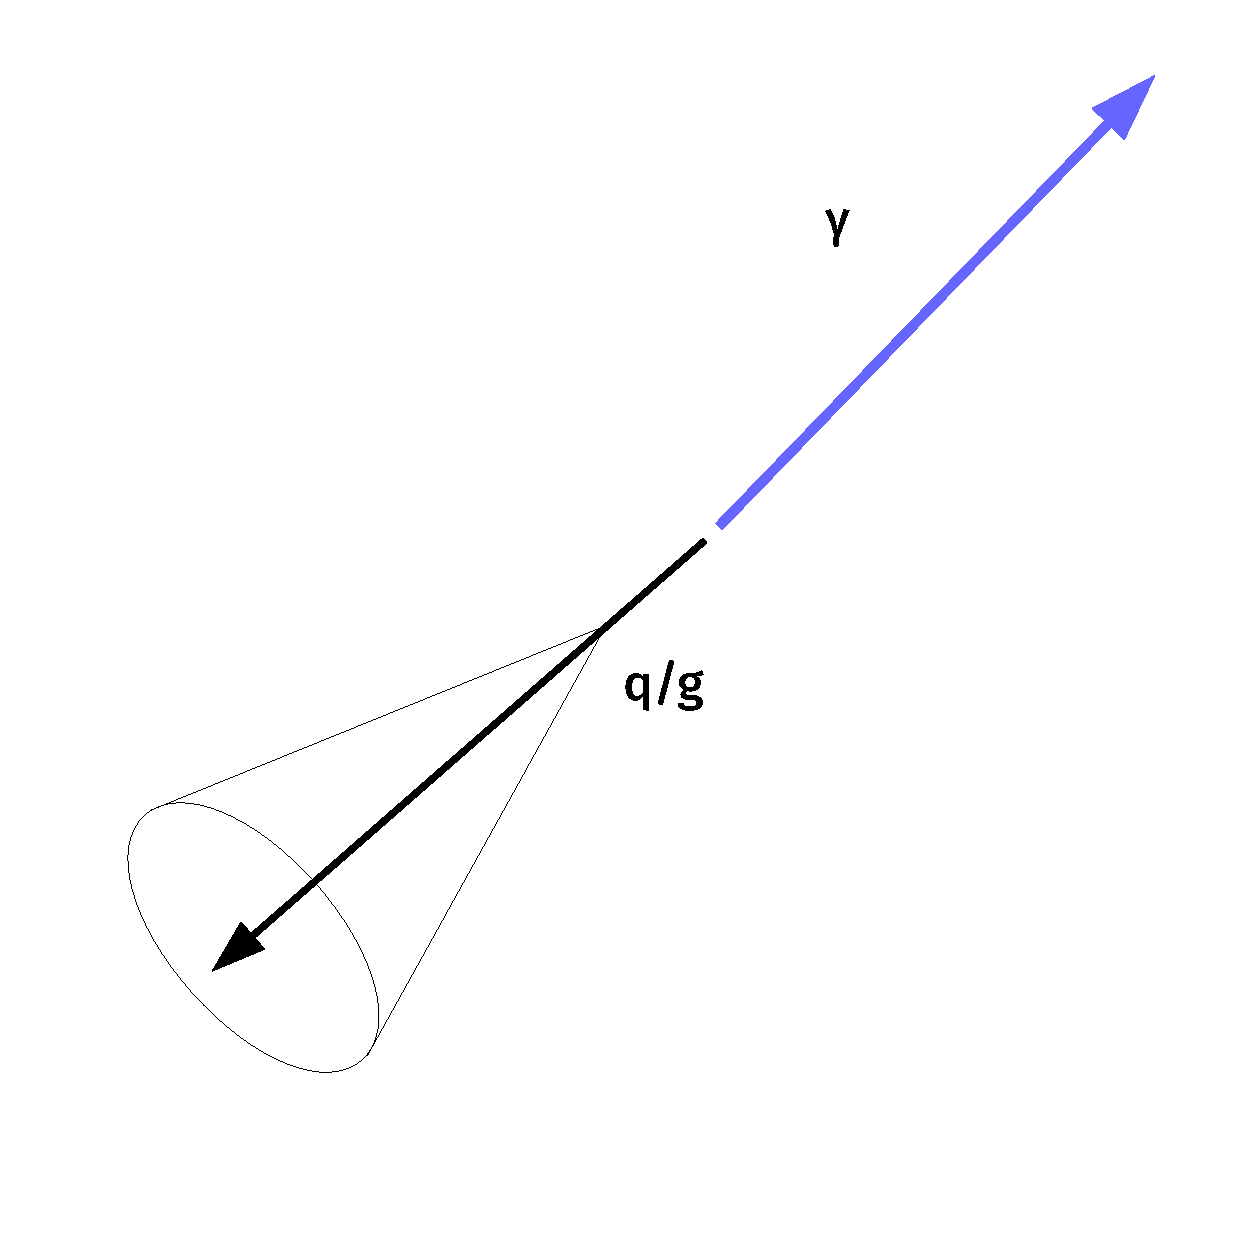
\includegraphics[width=1.5\textwidth]{figs/sketches/acr.pdf}};
%     \node(ttDiag) [right of=ttSR] {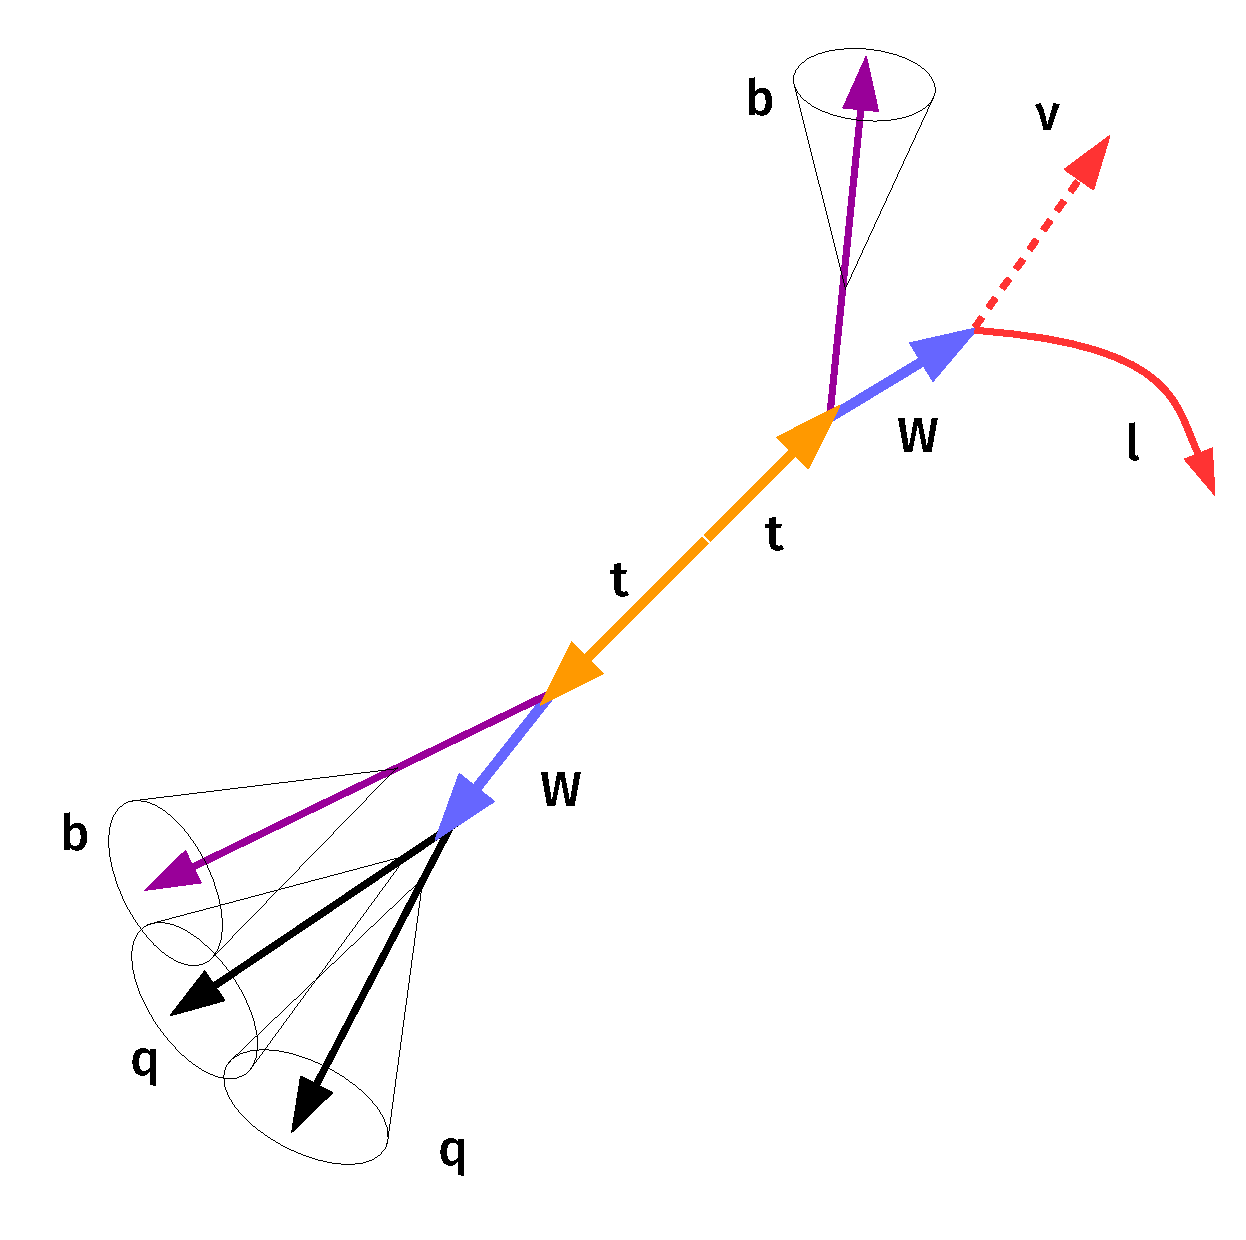
\includegraphics[width=1.5\textwidth]{figs/sketches/ttcr.pdf}};
% 
%     \path[dashed]
%           (ZvvSR) edge          node {} (ZllCR)
%           (WlvSR) edge          node {} (WlvCR)
%           (ttSR)  edge          node {} (tttCR)
%           (ttSR)  edge          node {} (ttWCR)
%     ;
%     \path
%           (ZvvSR) edge          node {} (ACR)
%           (ZvvSR) edge          node {} (WlvSR)
%     ;
%   \end{tikzpicture}
%   \end{minipage}
%   \put(-270,-45){Largest uncertainties:}
%   \put(-270,-60){- $\ell$ and $b$ ID }
%   \put(-270,-75){- $\gamma/Z$ and $W/Z$ prediction}
% \end{frame}
% 
% \begin{frame}[t]  \frametitle{Unblinding the data}
%   \begin{columns}
%   \begin{column}{0.25\textwidth}
%     \centering
%     Signal \\
%     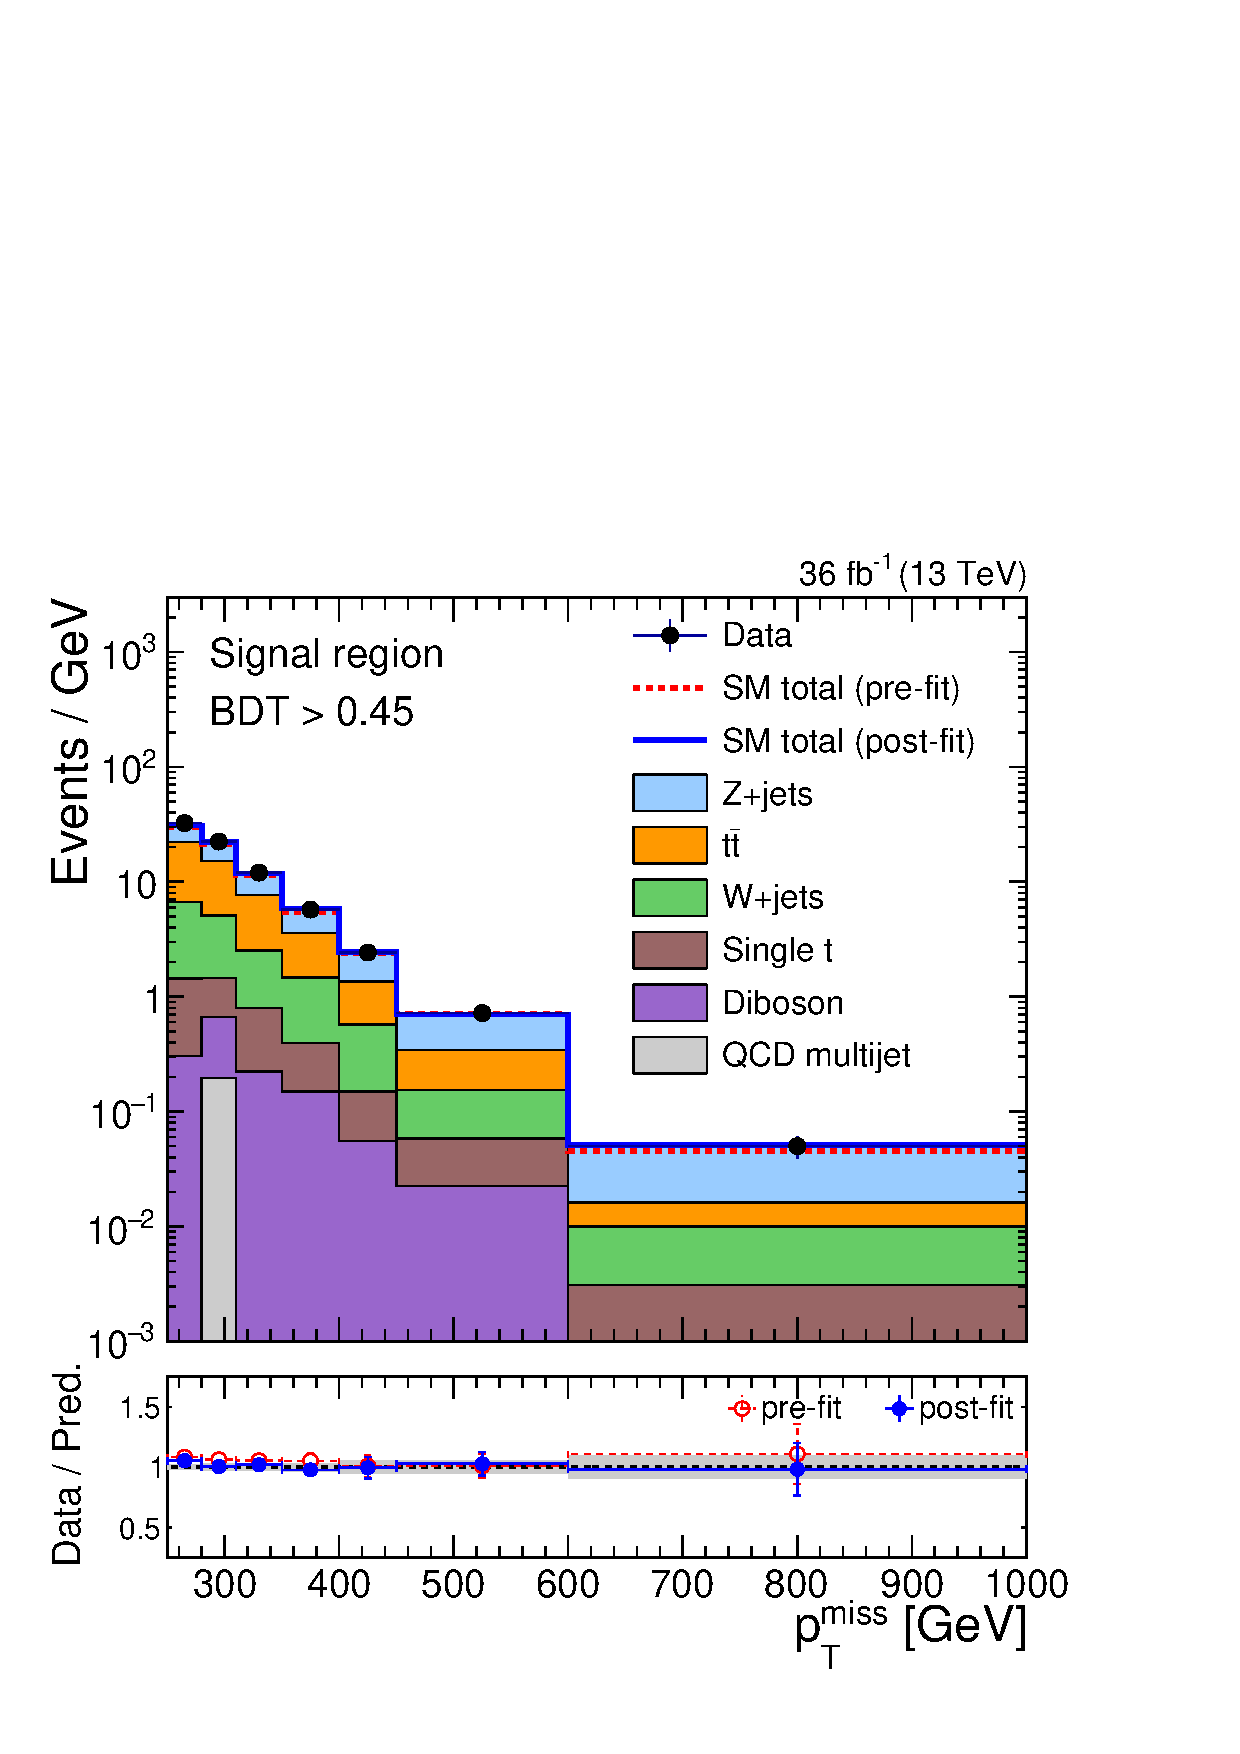
\includegraphics[width=\textwidth]{../../figs/monotop/v14/fr/brown/stackedPostfit_signal_monotop.pdf} \\
%   \end{column}
%   \begin{column}{0.25\textwidth}
%     \centering
%     $Z\rightarrow e e$ \\
%     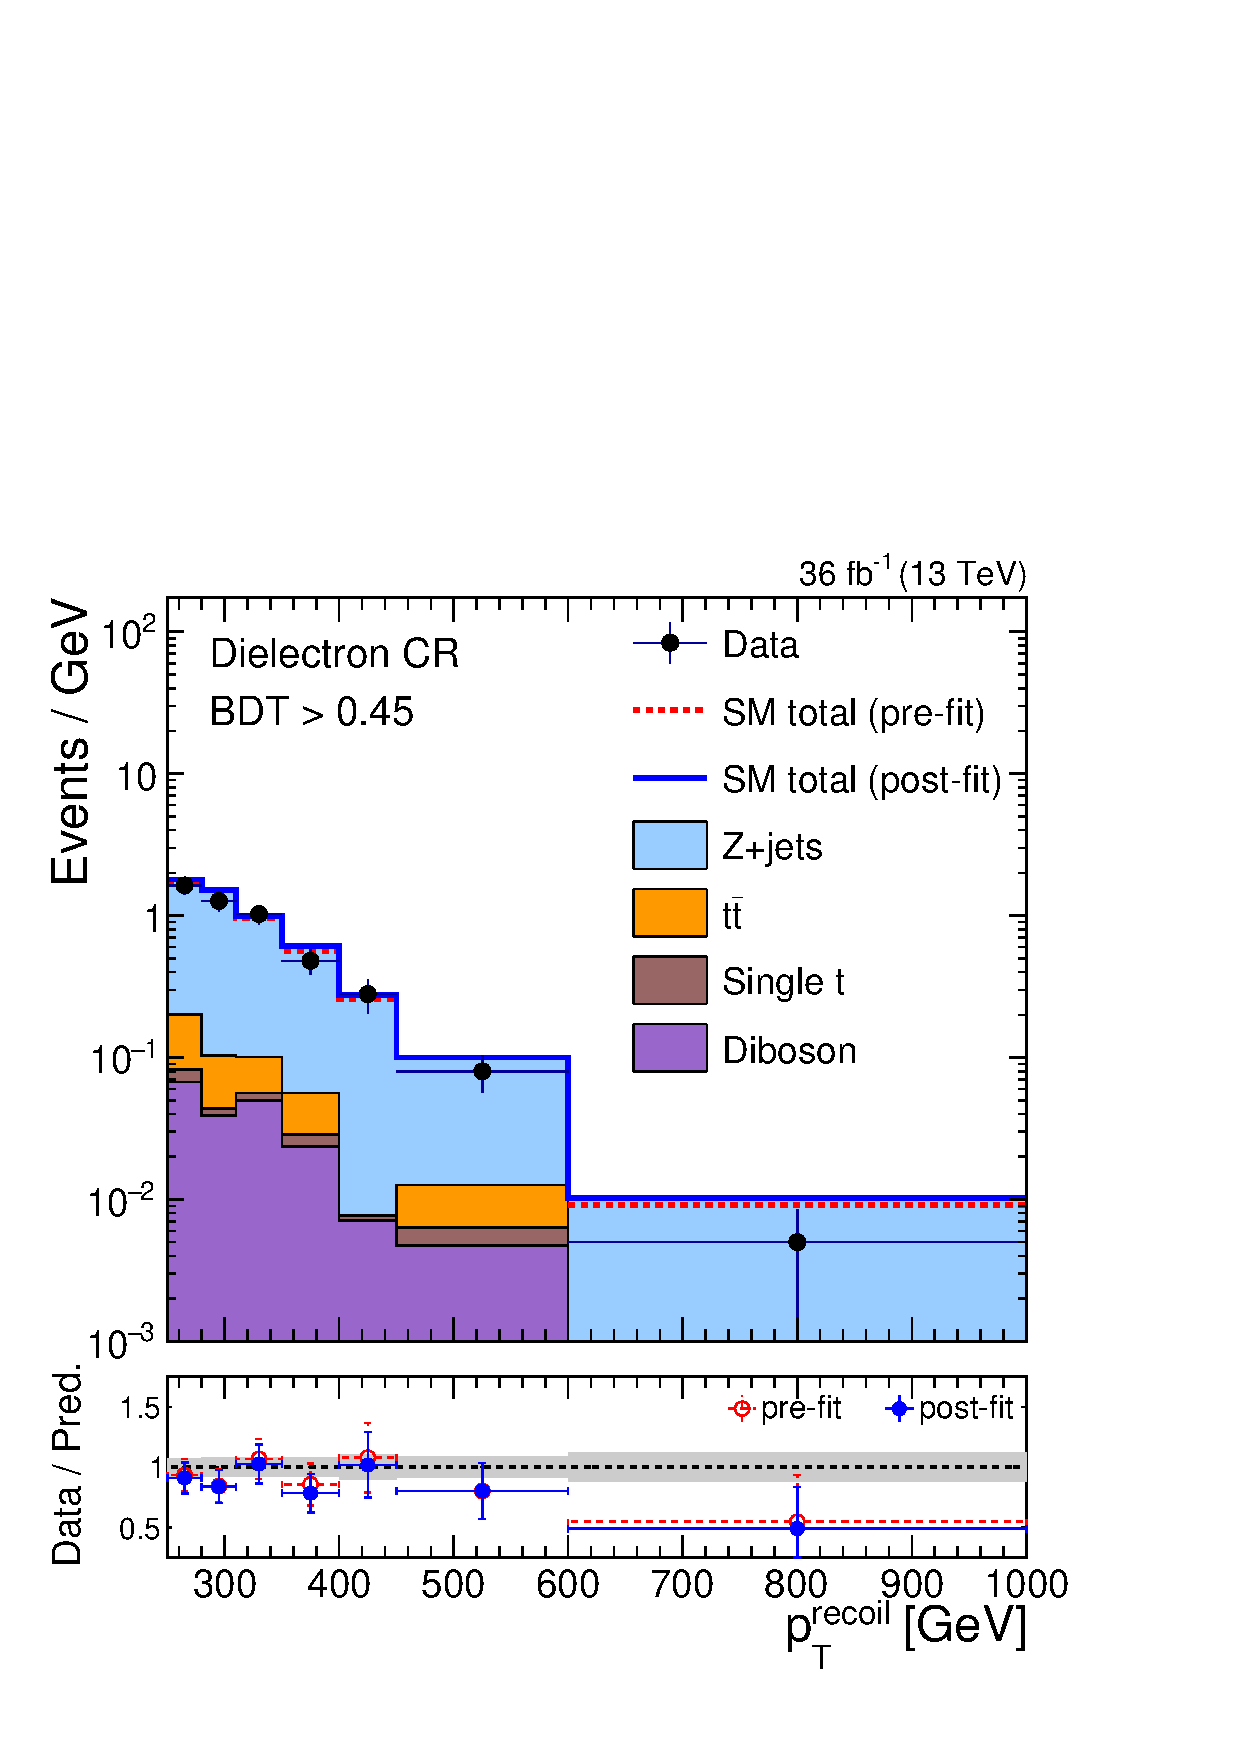
\includegraphics[width=\textwidth]{../../figs/monotop/v14/fr/brown/stackedPostfit_dielectron_monotop.pdf} \\
%   \end{column}
%   \begin{column}{0.25\textwidth}
%     \centering
%     $\gamma$ \\
%     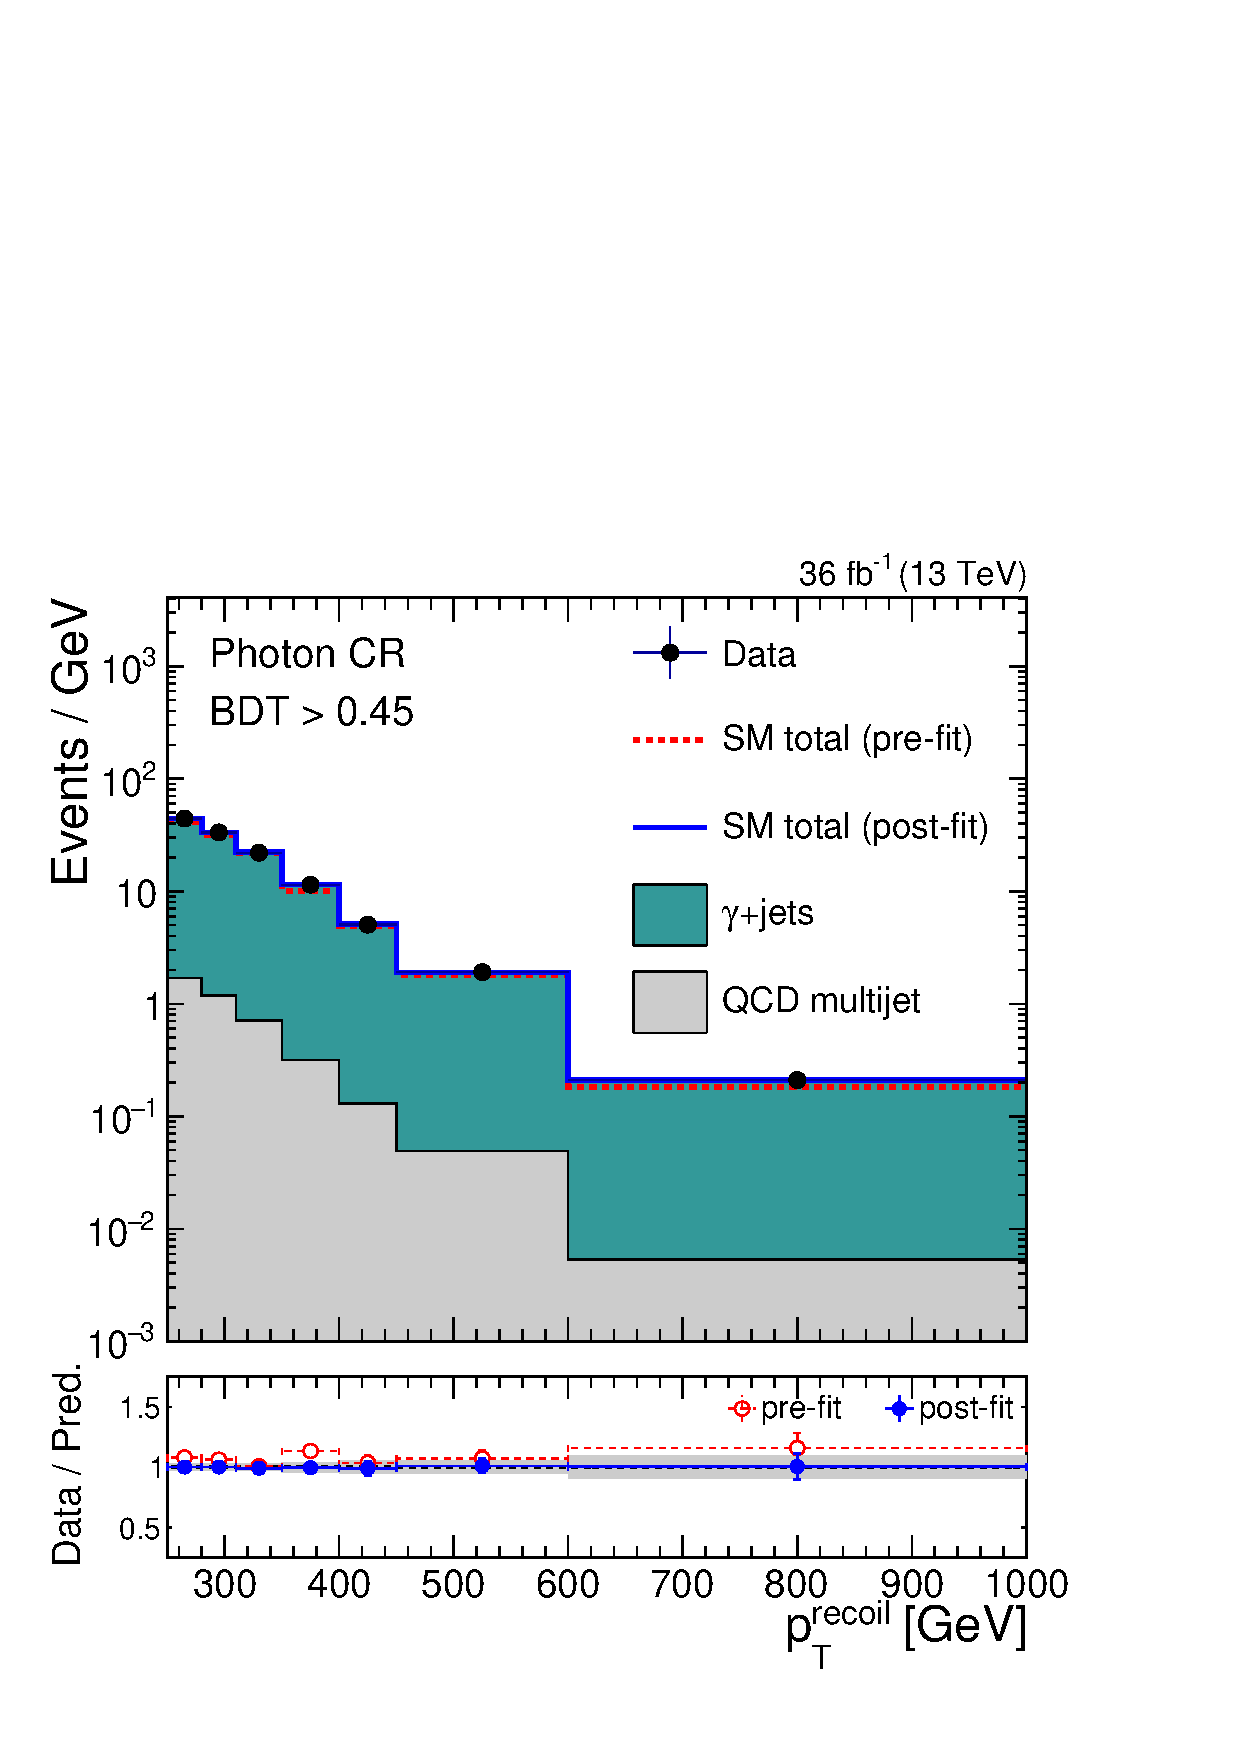
\includegraphics[width=\textwidth]{../../figs/monotop/v14/fr/brown/stackedPostfit_photon_monotop.pdf} \\
%   \end{column}
%   \begin{column}{0.25\textwidth}
%     \centering
%     $ t\bar{t}\rightarrow  \mu\nu$+jets \\
%     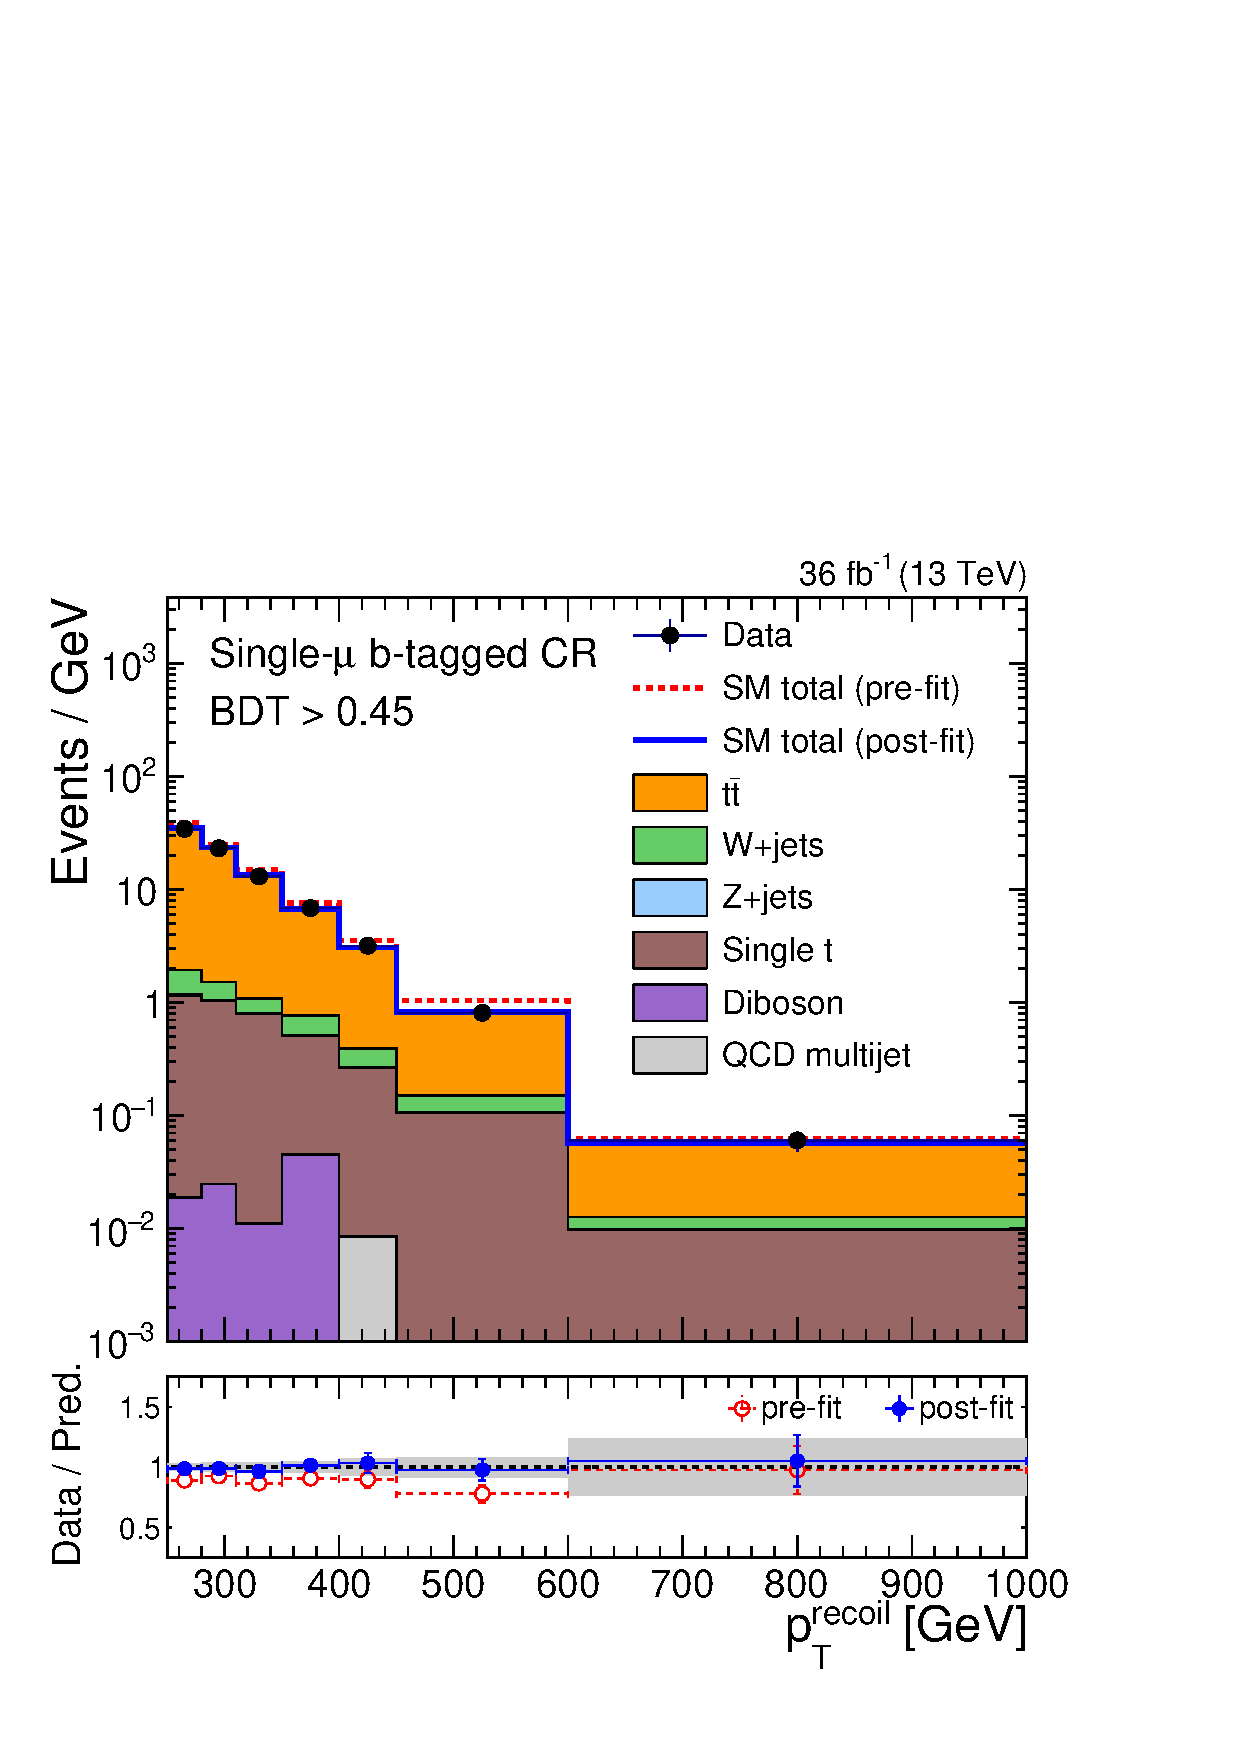
\includegraphics[width=\textwidth]{../../figs/monotop/v14/fr/brown/stackedPostfit_singlemuontop_monotop.pdf} \\
%   \end{column}
%   \end{columns}
% 
%   \begin{itemize}
%     \item Too many regions to show all here
%     \item SM processes are able to describe data quite well in all regions, including the SRs
%     \item No observation of an excess
%   \end{itemize}
% \end{frame}
% 
% \begin{frame}[t]   \frametitle{No observation? Set limits}
%   \vspace{-5mm}
%   \centering
%     Benchmark models probe different mono-top kinematics.
%     \vspace{3mm}
%   \begin{columns}
%   \begin{column}{0.5\textwidth}
%     \centering
%       Resonant scalar
%     \begin{itemize}
%       \item $\pt$ of top quark increases with $m_\phi$
%       \item Therefore, efficiency of signal selection improves at high $m_\phi$
%     \end{itemize}
%     \centering
%     \only<1>{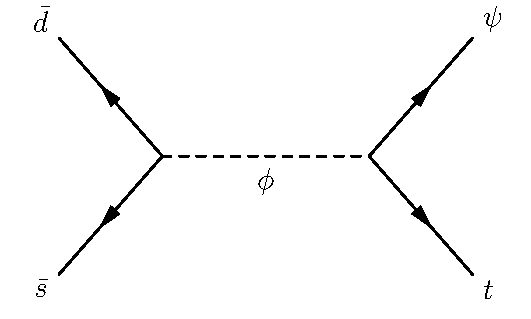
\includegraphics[width=0.8\textwidth]{figs/feynman/resonant.pdf}}
%     \only<2>{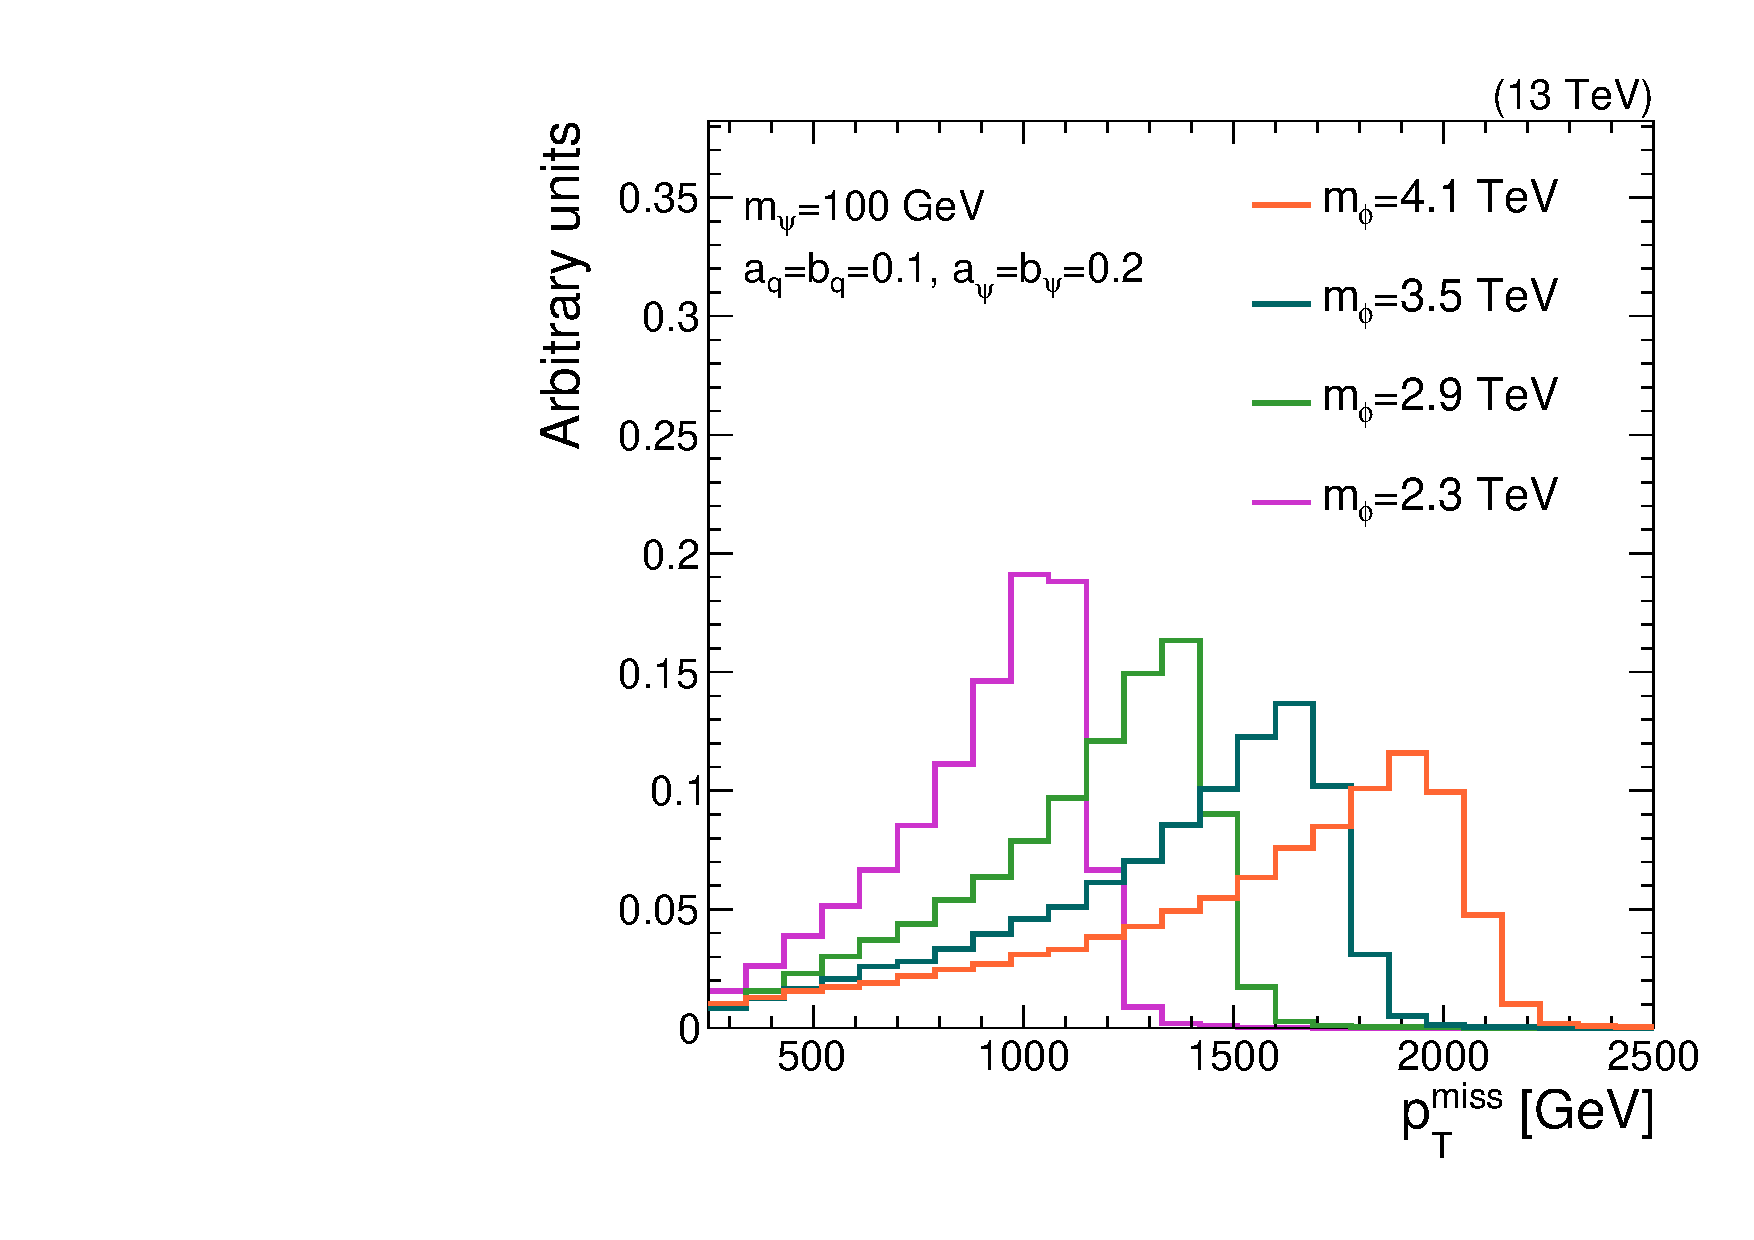
\includegraphics[width=0.6\textwidth]{../../figs/monotop/v14/cwr/jandrea/res_pfmet.pdf}}
%     \only<3>{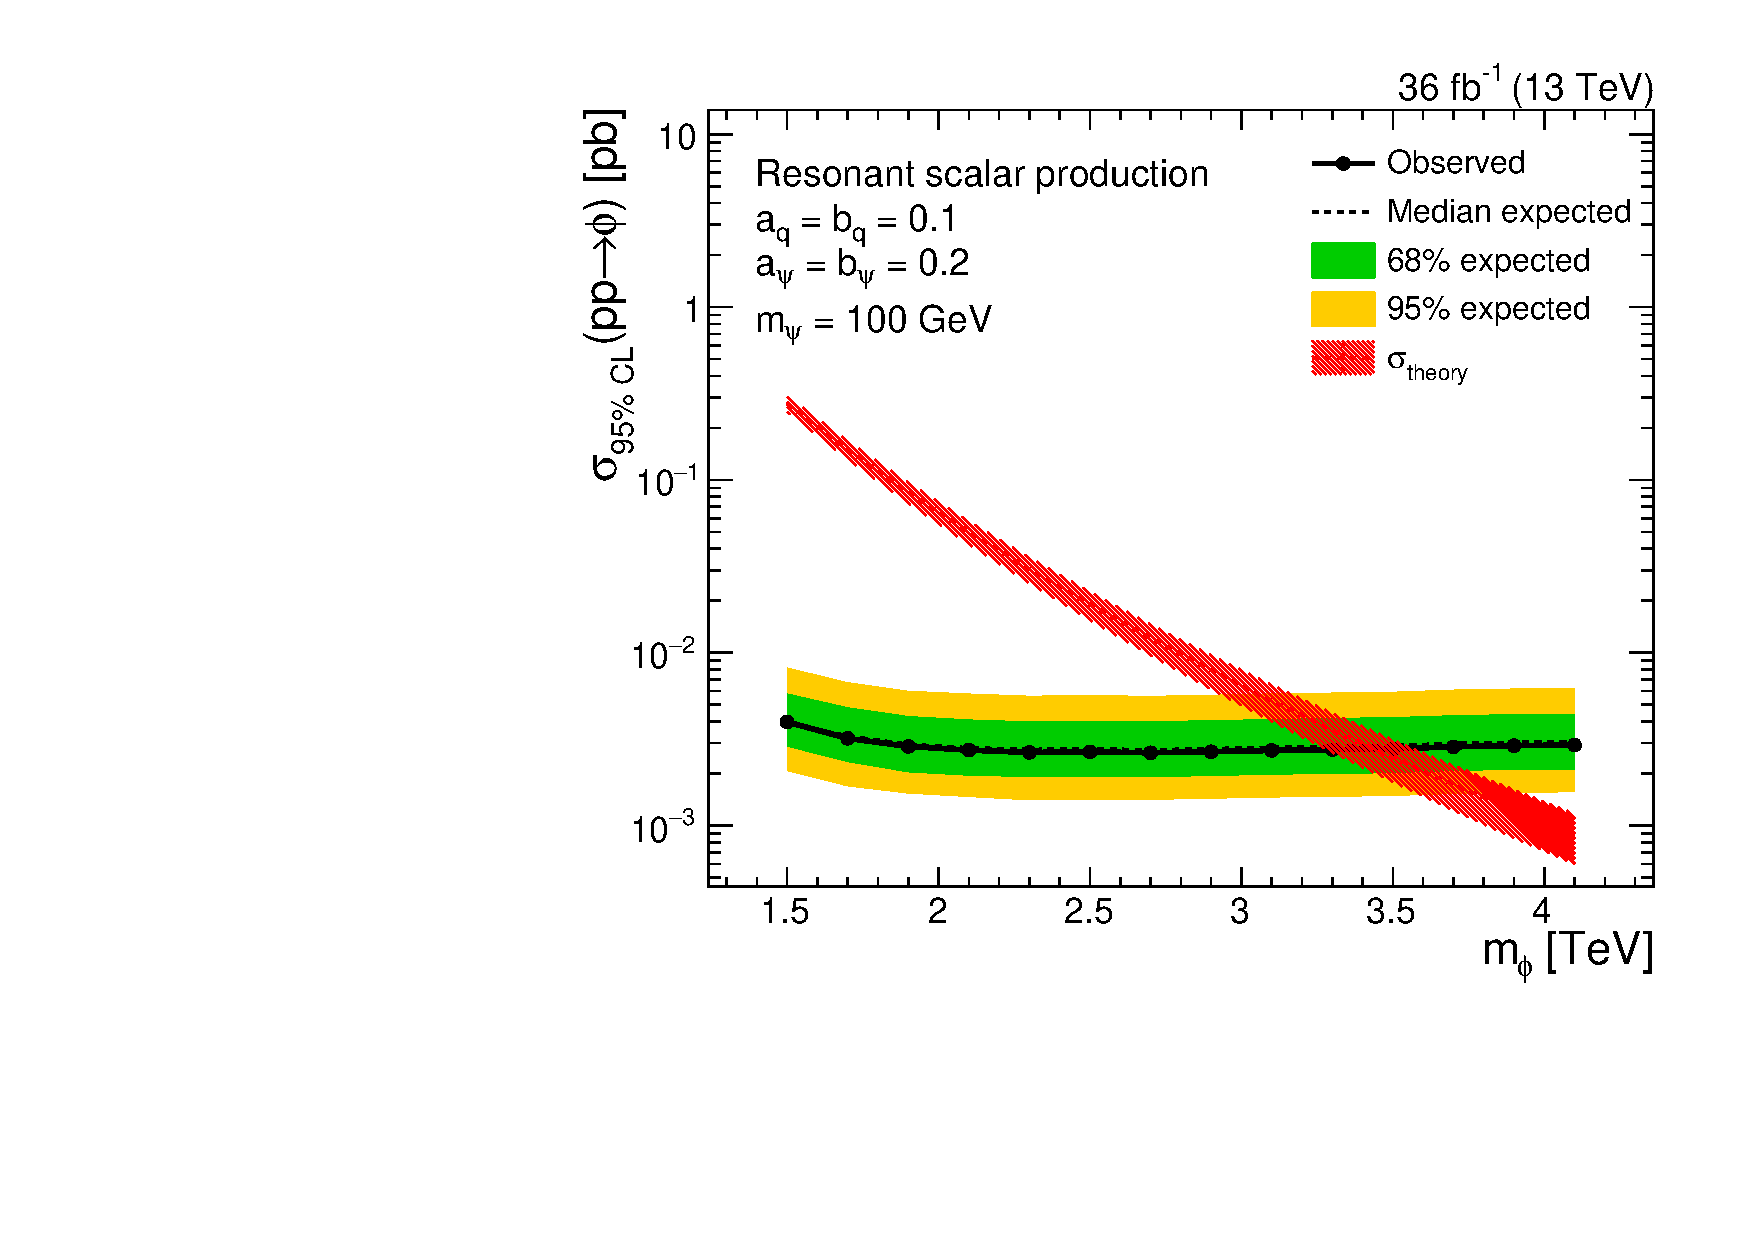
\includegraphics[width=0.7\textwidth]{../../figs/monotop/v14/fr/colors/res_obs_limit.pdf}}
%   \end{column}
%   \begin{column}{0.5\textwidth}
%     \centering
%       FCNC
%     \begin{itemize}
%       \item Falling $\ptmiss$ spectra $\Rightarrow$ worse signal eff.
%       \item Interesting parameters to constrain are $m_V$ and couplings $g_\chi, g_q$
%     \end{itemize}
%     \centering
%     \only<1>{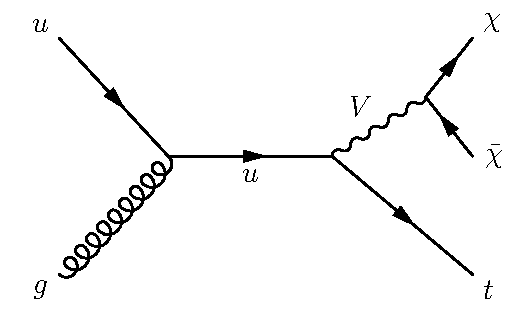
\includegraphics[width=0.8\textwidth]{figs/feynman/fcncb.pdf}}
%     \only<2>{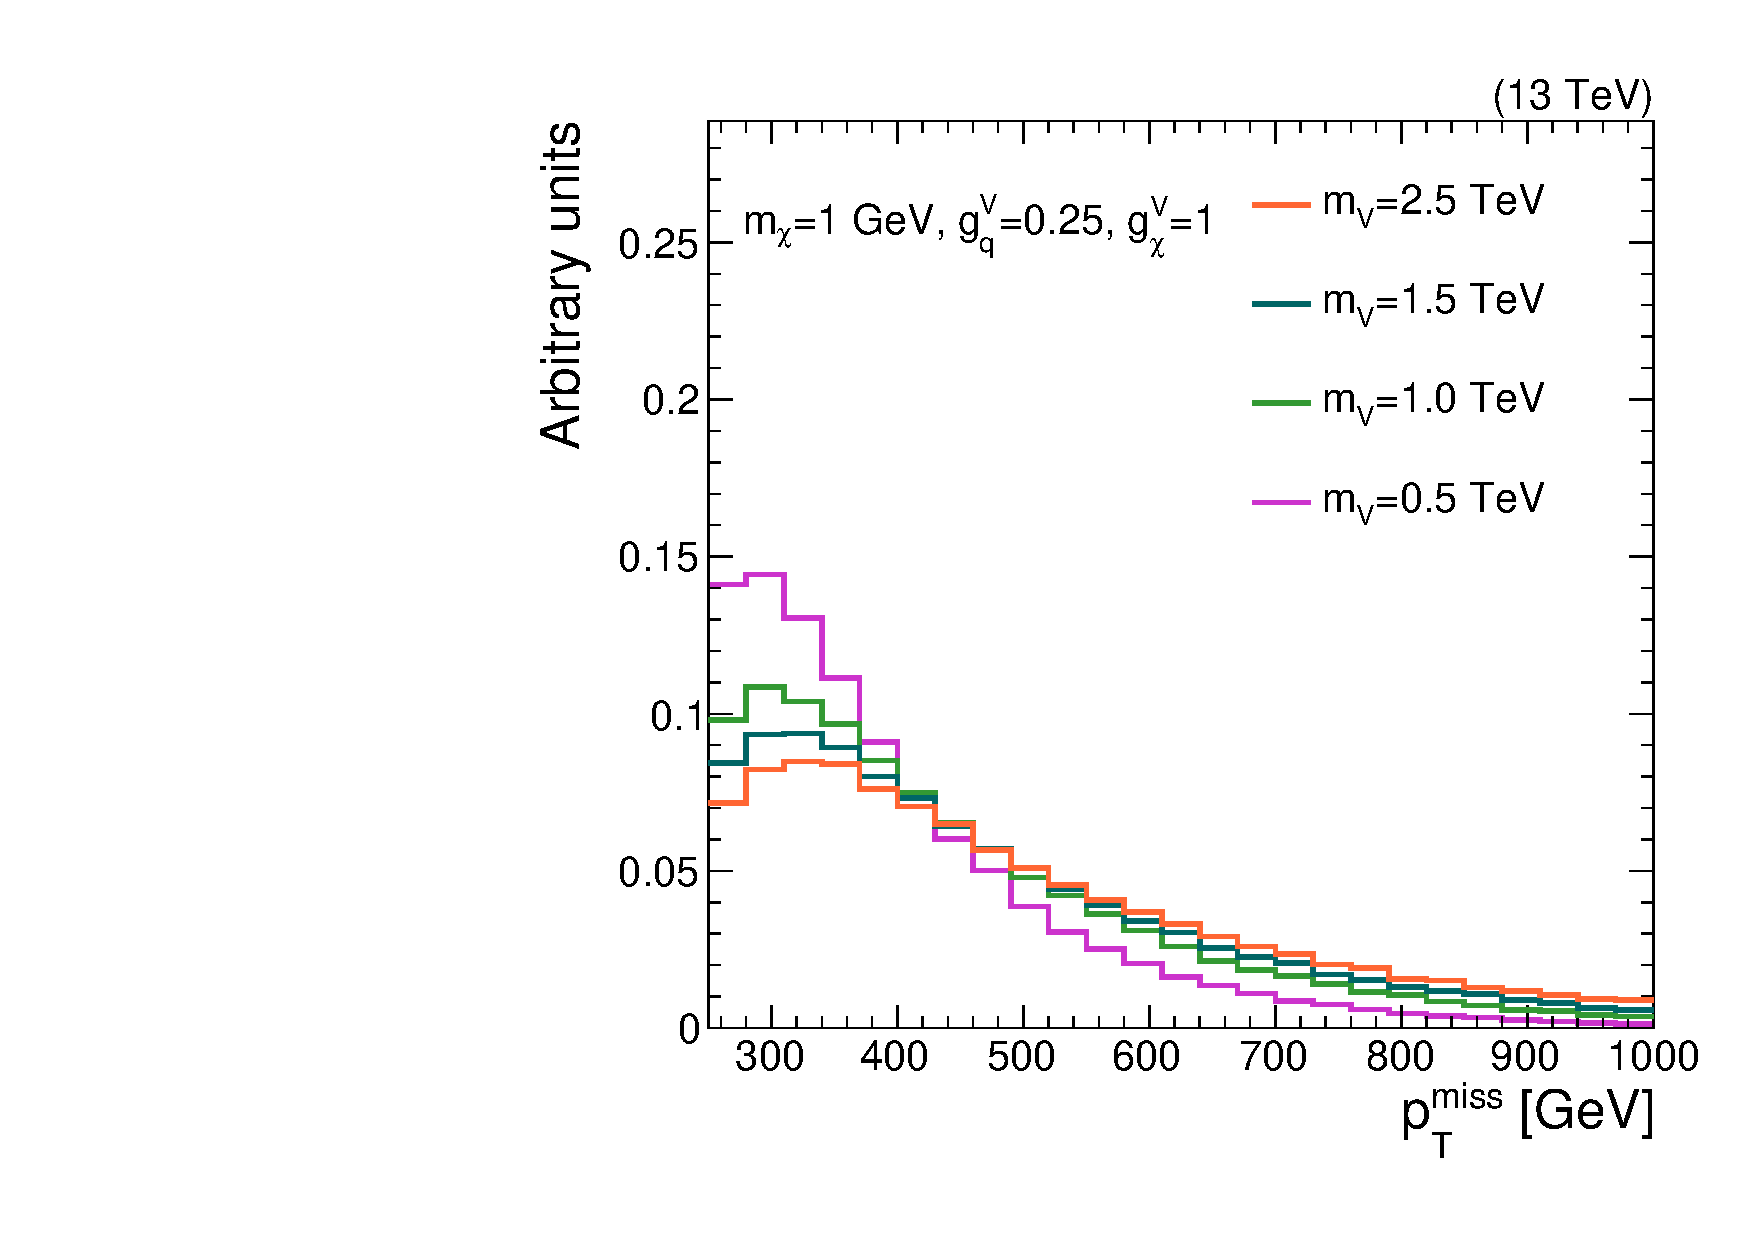
\includegraphics[width=0.6\textwidth]{../../figs/monotop/v14/cwr/jandrea/fcnc_pfmet.pdf}}
%     \only<3>{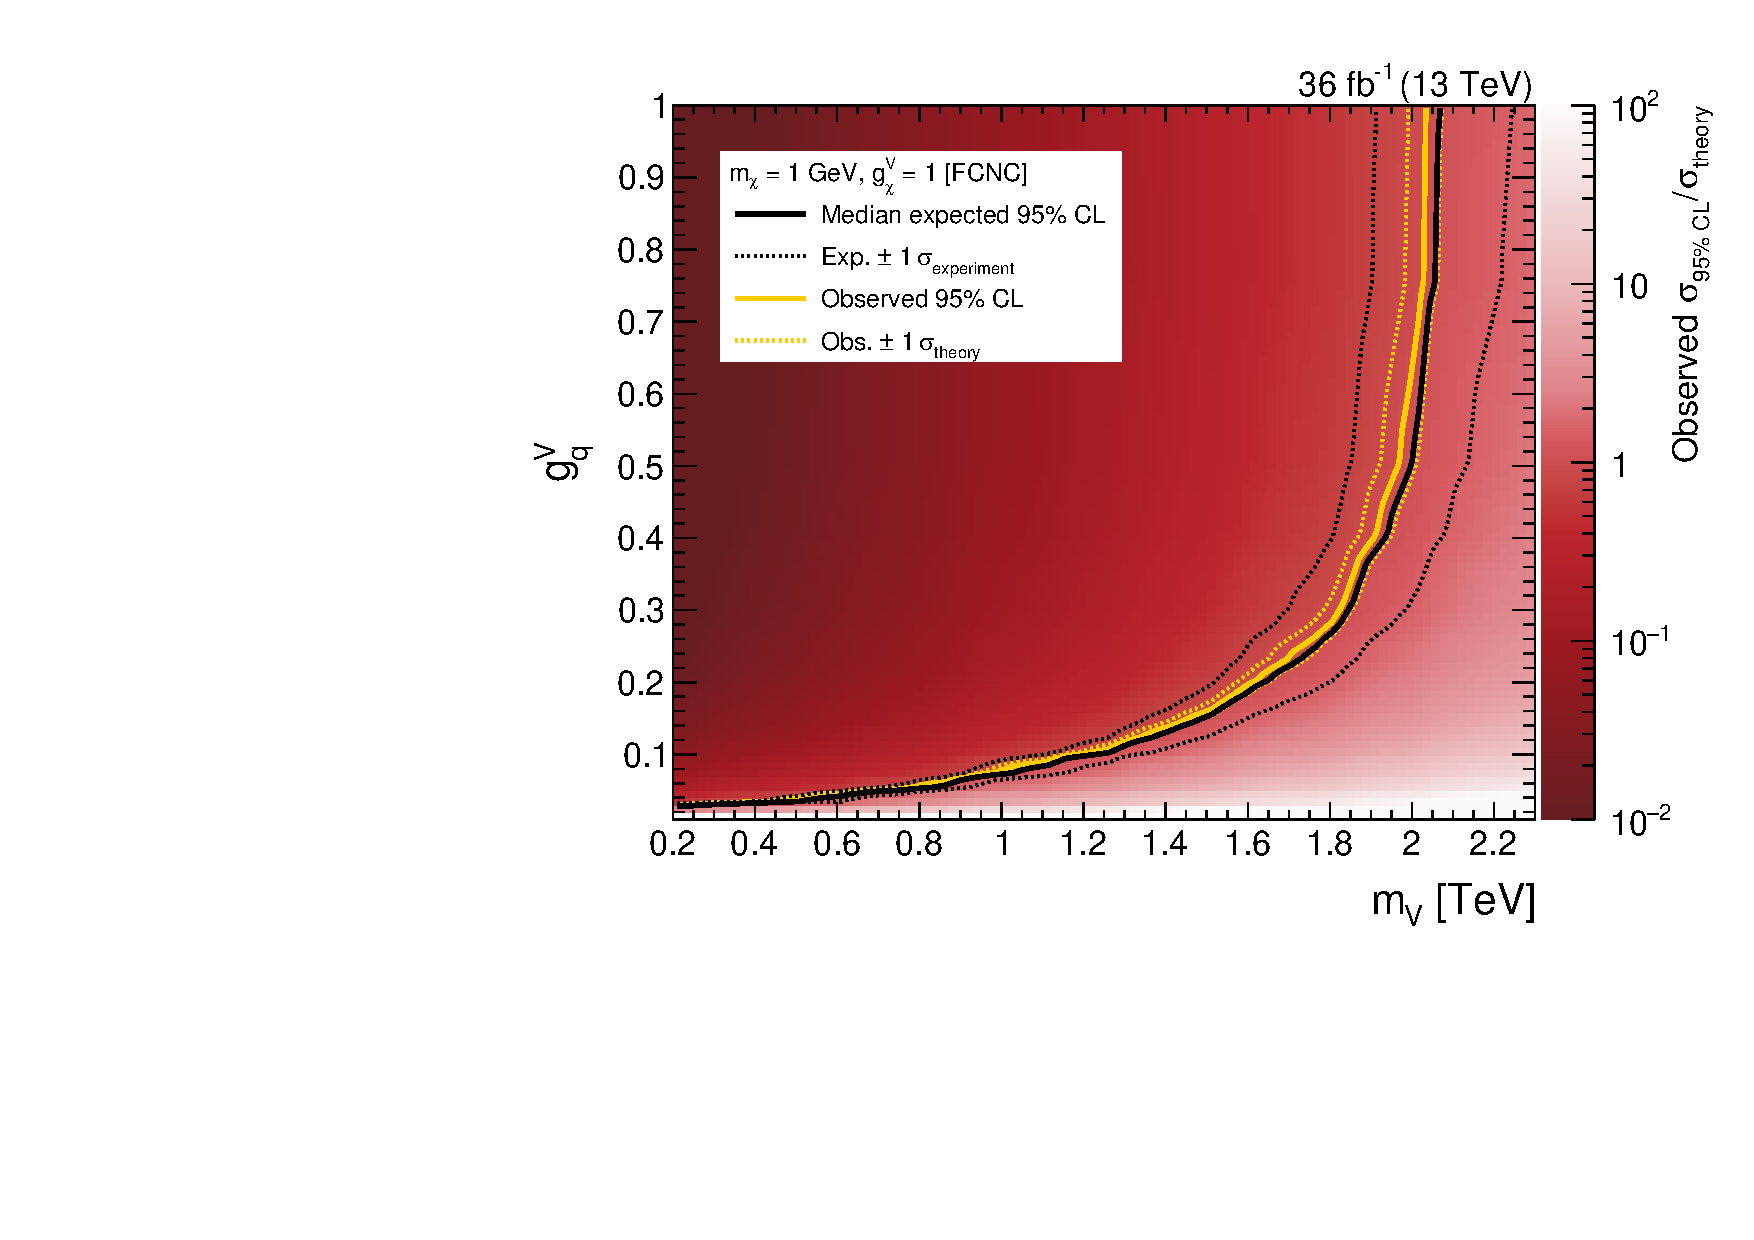
\includegraphics[width=0.7\textwidth]{../../figs/monotop/v14/fr/colors/fcnc2d_obs_gqv_mV.pdf}}
%   \end{column}
%   \end{columns}
% \end{frame}
% 
% \begin{frame} \frametitle{Another DM+substructure search: mono-Higgs($bb$)}
%   \vspace{-5mm}
%   \begin{columns}[T]
%     \begin{column}{0.6\textwidth}
%       \begin{itemize}
%         \item Backgrounds and estimation technique very similar to mono-top
%         \item Sensitive to extended Higgs sectors (2HDM+a, baryonic $Z'$,\dots)
%         \item Replace 3-prong/1-$b$ with 2-prong/2-$b$ large-radius jet
%       \end{itemize}
%     \end{column}
%     \begin{column}{0.4\textwidth}
%       \centering
%       \includegraphics[width=0.6\textwidth]{figs/monoh/Feyn-2HDMa.pdf}
%     \end{column}
%   \end{columns}
%   \centering
%         \includegraphics[width=0.65\textwidth]{figs/monoh/fatjet.pdf}
%         \includegraphics[width=0.35\textwidth]{figs/monoh/limits_2hdma_mass_prelim.pdf}
% \end{frame}
% 
% \begin{frame} \frametitle{Detour: ML for substructure}
%   \vspace{-5mm}
%   \begin{itemize}
%     \item Top-tagging using QCD-motivated observables works very well
%     \item Are we reaching a ``maximum'' performance threshold?
%     \item One approach is to \textcolor{maroon}{brute-force the problem using deep learning}
%     \item Factorize the question: physics effects vs. detector effects
%     \item Following studies are done using \textcolor{maroon}{hadron-level simulation}
%     \begin{itemize}
%       \item Madgraph5 at LO for hard scattering
%       \item Pythia8 for hadronization
%       \item No detector simulation
%     \end{itemize}
%      \item Training is done on a desktop computer
%      \begin{itemize}
%        \item NVIDIA GTX 1080 GPU
%        \item Keras\footnote{\url{https://github.com/keras-team/keras}} with tensorflow\footnote{\url{https://github.com/tensorflow/tensorflow}} backend
%      \end{itemize}
%   \end{itemize}
% \end{frame}
% 
% \begin{frame}[t]  \frametitle{Observables}
%   \begin{minipage}{\textwidth}
%   \begin{itemize}
%      % \item Jet definition more commonly used at LHC:
%      % \begin{itemize}
%      %   \item $\pt>400\,\gev$
%      %   \item Anti-$k_\mathrm{T}$, $R=0.8$
%      % \end{itemize}
%      \item For each particle in the jet, 7 features:
%      \begin{itemize}
%        \item $p^\mu$
%        \item $\Delta R($particle,jet$)$
%        \item Soft drop survival
%        \item Particle type ($e^\pm$, $\mu^\pm$, $\gamma$, charged hadron$^\pm$, neutral hadron)
%      \end{itemize}
%      \item Rotate the jet so:
%      \begin{itemize}
%        \item Jet axis coincides with $z$-axis
%        \item Hardest particle away from jet axis lies in $x$-$z$ plane
%      \end{itemize}
%    \end{itemize}
%   \end{minipage}
%   \put(-130,-100){\includegraphics[width=0.3\textwidth]{figs/jet_rot.png}}
% \end{frame}
% 
% \begin{frame}[t] \frametitle{Network architectures}
%   \vspace{-7mm}
%   \begin{columns}[T]
%     \begin{column}{0.7\textwidth}
%       \only<1>{\includegraphics[width=\textwidth,page=1]{figs/flowcharts.pdf}}
%       \only<2>{\includegraphics[width=\textwidth,page=2]{figs/flowcharts.pdf}}
%       \only<3>{\includegraphics[width=\textwidth,page=3]{figs/flowcharts.pdf}}
%     \end{column}
%     \begin{column}{0.3\textwidth}
%       - Fully connected: brute force approach \\
%       \vspace{5mm}
%       \uncover<2->{- Recurrent NN: read the jet as a ``sentence'', where a particle is a ``word''\\}
%       \vspace{5mm}
%       \uncover<3->{- 1D convolutions: allows some invariance to incorrect ordering}
%     \end{column}
%   \end{columns}
% \end{frame}
% 
% \begin{frame}[t]  \frametitle{DNN performance}
%   \vspace{-7mm}
%   \begin{columns}
%   \begin{column}{0.5\textwidth}
%   \begin{itemize}
%     \item Compare fully-connected network to ``shallow'' network using ECFs
%     \item $\mathcal{O}(10^6)$ parameters
%     \item Positive: performant classifier without thinking about physics
%     \item Negative: that's it?
%     \uncover<2->{
%     \item Dramatic improvement from giving structure to the network
%     \item Adding more information ($4\rightarrow7$) or more particles ($50\rightarrow100$) helps
%     \item C-LSTMs have $\mathcal{O}(10^5)$ parameters
%     }
%   \end{itemize}
%   \end{column}
%   \begin{column}{0.5\textwidth}
%   \begin{center}
%     \only<1>{\includegraphics[width=\textwidth,page=1]{../../figs/deepgen/v4_dense/roc.pdf}}
%     \only<2>{\includegraphics[width=\textwidth,page=1]{../../figs/deepgen/v4/roc.pdf}}
%   \end{center}
%   \end{column}
%   \end{columns}
% \end{frame}
% 
% \begin{frame} \frametitle{Next steps/WIP}
%   \begin{itemize}
%     \item Quantifying how realistic this improvement is
%     \begin{itemize}
%       \item What are we learning that QCD observables don't capture?
%       \item Is it IRC unsafe things?
%       \item How does detector smearing hurt?
%       \begin{itemize}
%         \item Hint: it's painful
%       \end{itemize}
%     \end{itemize}
%     \pause
%     \item Removing correlation with various nuisances
%     \begin{itemize}
%       \item Kinematics of jet: mass, $\pt$
%       \item Pile-up
%       \item QCD uncertainties
%       \begin{itemize}
%         \item Again, IRC unsafety plays a role
%       \end{itemize}
%     \end{itemize}
%     \pause
%     \item There is a lot of promise in these approaches!
%   \end{itemize}
% \end{frame}
% 
% \secpage{VBF $H\rightarrow$ invisible}
% 
% \begin{frame} \frametitle{Invisible Higgs}
%     \vspace{-3mm}
%       \begin{itemize}
%         \item DM fermion could be given mass through Higgs mechanism
%         \item If $2m_\chi < m_H$, should observe $H\rightarrow\chi\bar\chi$
%         \item Production mode $\Rightarrow$  mono-\X~channels
%         \begin{itemize}
%           \item $gg\rightarrow H$ + ISR $\Rightarrow$ mono-jet
%           \item $VH$ $\Rightarrow$ mono-$V(qq')$ and mono-$Z(\ell\ell)$
%           \item VBF $\Rightarrow$ VBF+$H\rightarrow$inv
%         \end{itemize}
%       \end{itemize}
%       \centering
%       \includegraphics[width=1\textwidth]{figs/diagrams/hinv.png}
% \end{frame}
% 
% \begin{frame}   \frametitle{VBF production of bosons}
%   \vspace{-5mm}
%   \begin{columns}
%     \begin{column}{0.33\textwidth}
%       Characterized by:
%       \begin{itemize}
%         \item Two forward jets
%         \item Large $\pt^{H}$
%       \end{itemize}
%       Can replace $H$ with $Z$ or $W$
%       \begin{itemize}
%         \item Irreducible background
%       \end{itemize}
%     \end{column}
%     \begin{column}{0.33\textwidth}
%       \centering
%       \includegraphics[width=\textwidth]{figs/diagrams/vbf_FD.pdf} \\
%       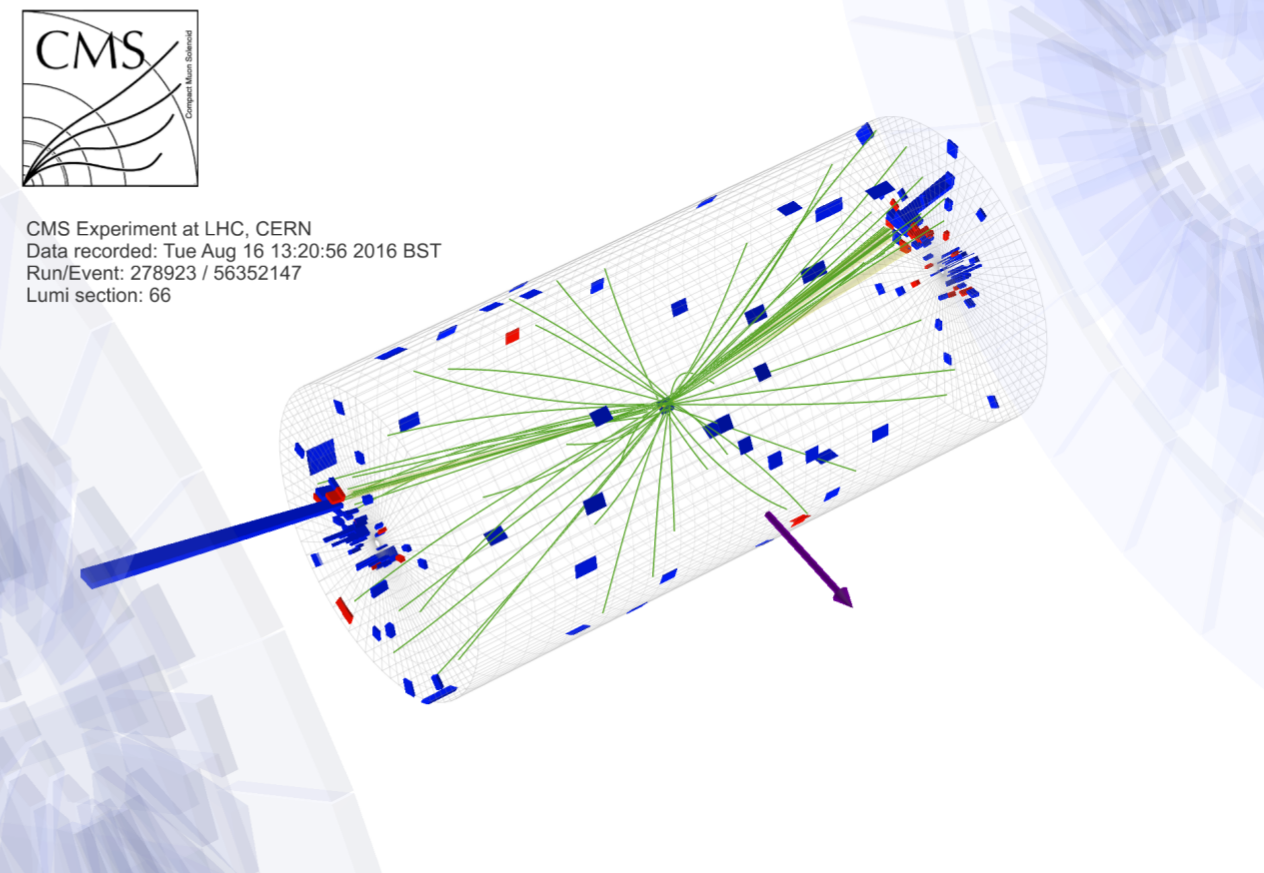
\includegraphics[width=1.2\textwidth]{figs/vbf/event_display.png}
%     \end{column}
%     \begin{column}{0.33\textwidth}
%       \centering
%       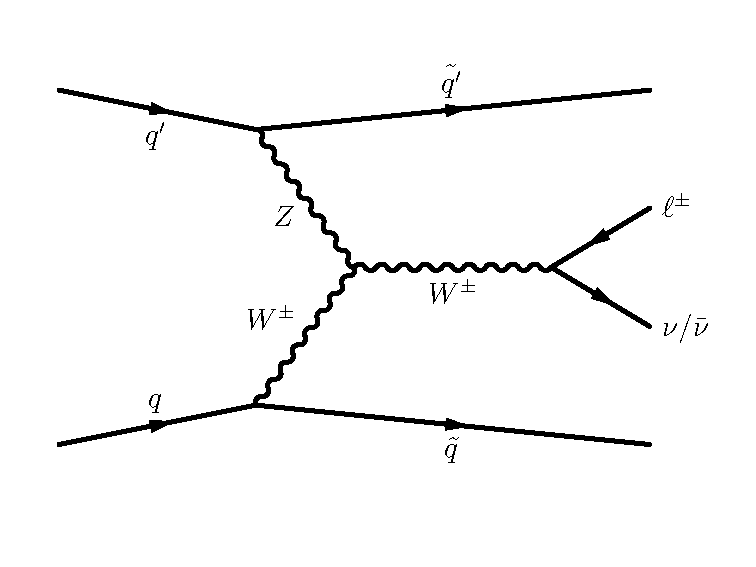
\includegraphics[width=\textwidth]{figs/diagrams/vbf_w.pdf} \\
%       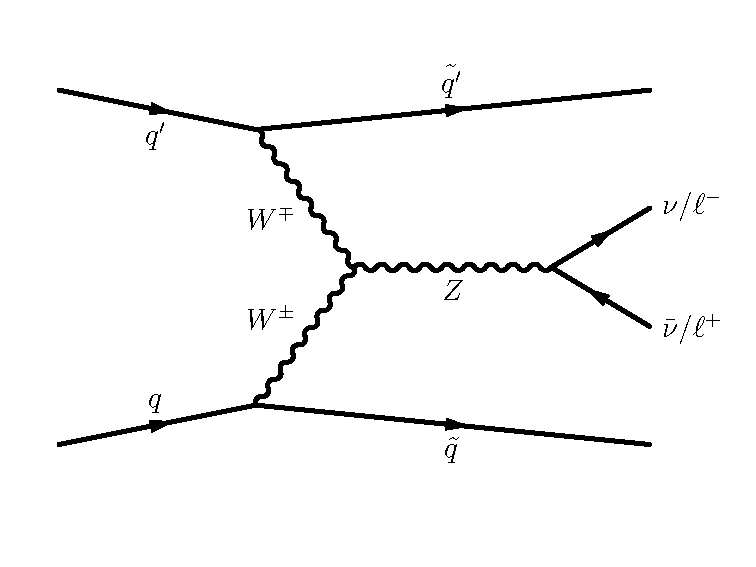
\includegraphics[width=\textwidth]{figs/diagrams/vbf_z.pdf}
%     \end{column}
%   \end{columns}
% \end{frame}
% 
% \begin{frame}   \frametitle{Forward jets are important}
%   \begin{itemize}
%     \item As with mono-top and mono-Higgs, we use the jets to mitigate backgrounds
%     \item In this case, the jets can be resolved distinctly
%   \end{itemize}
%   \centering
%   \includegraphics[width=0.33\textwidth]{figs/vbf/signal_jot12DEta.pdf}
%   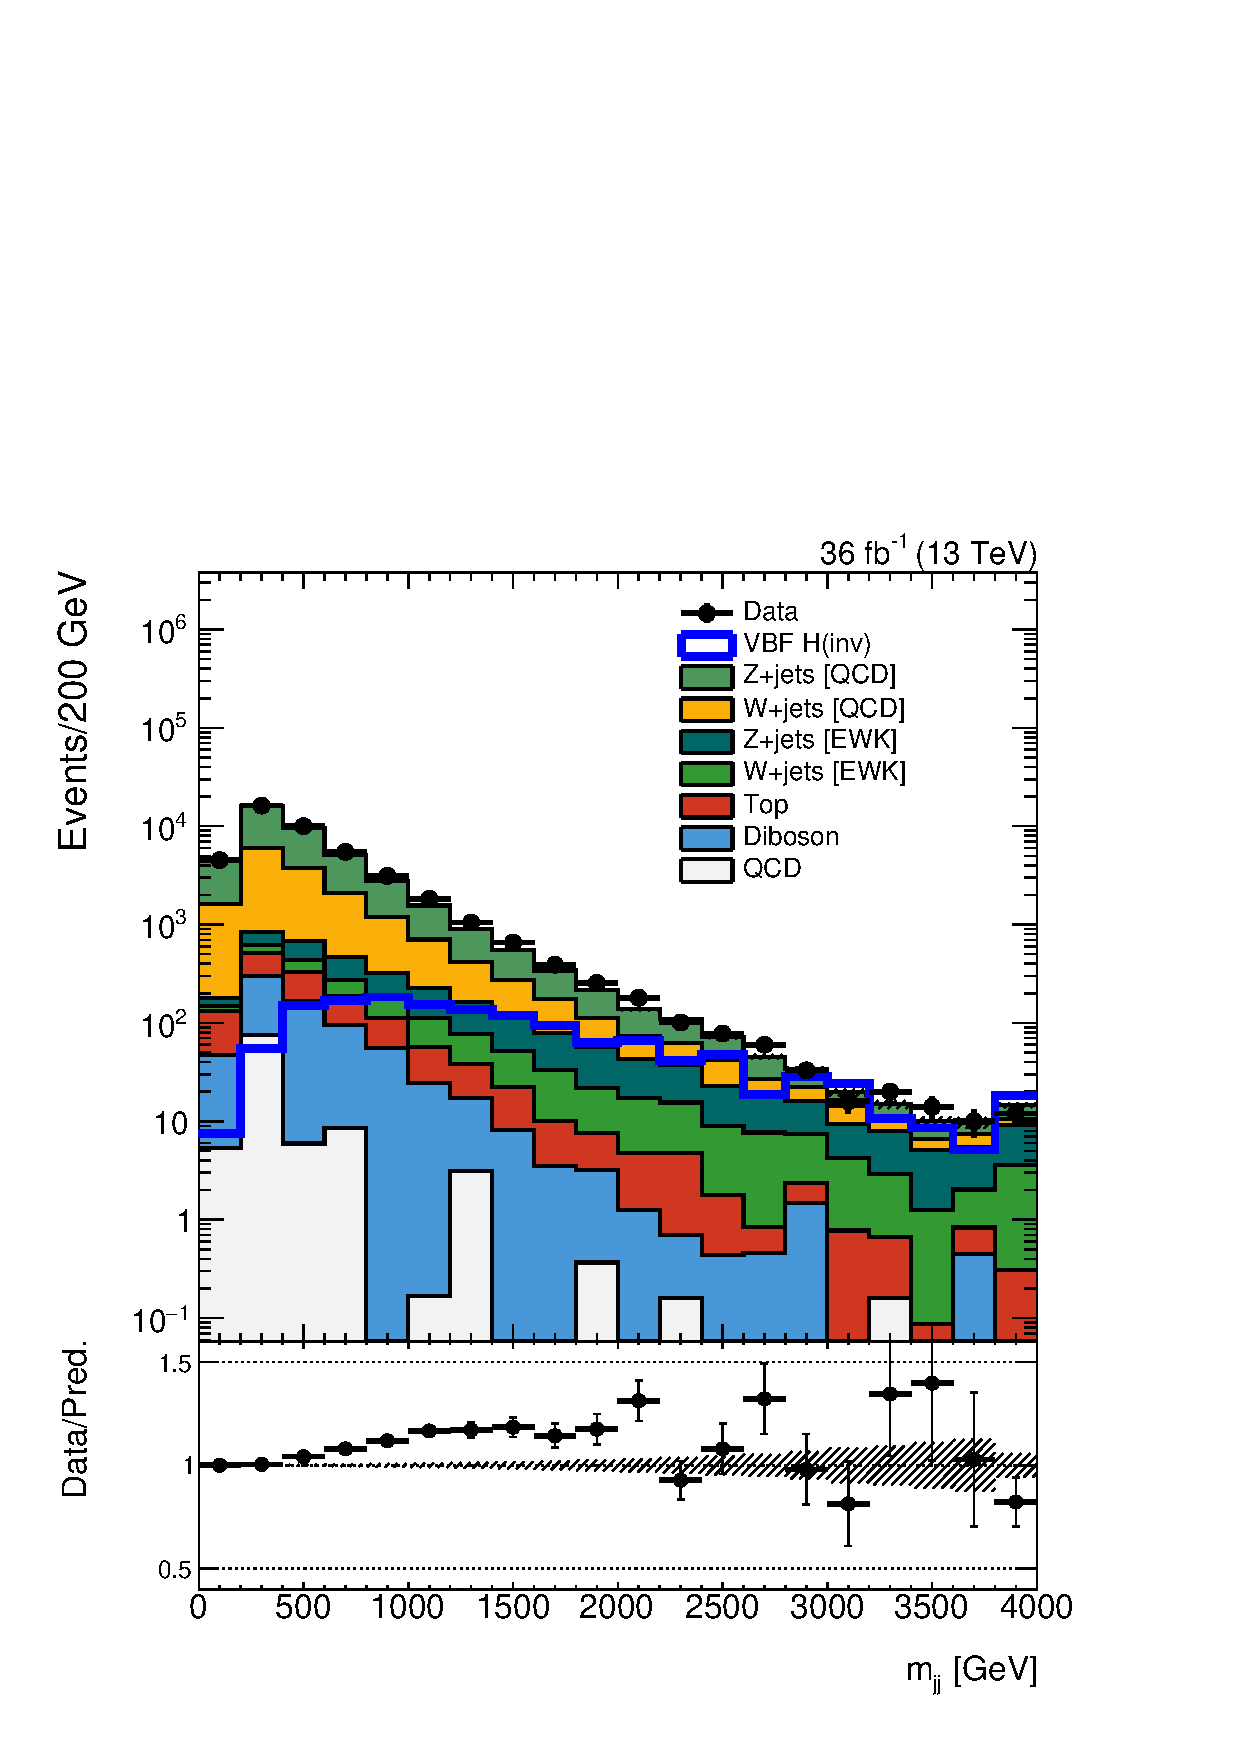
\includegraphics[width=0.33\textwidth]{figs/vbf/signal_jot12Mass_logy.pdf}
%   \includegraphics[width=0.33\textwidth]{figs/vbf/signal_jot12DPhi.pdf}
% \end{frame}
% 
% \begin{frame} \frametitle{Forward jets are challenging}
%   \vspace{-5mm}
%   \begin{itemize}
%     \item ``Forward'' typically refers to jets outside of the tracker's acceptance
%     \item Rely entirely on calorimeters
%     \item Energy resolution and trigger efficiency degrade in this region
%     \only<2> {\item Characterize events using quality within tracker acceptance}
%   \end{itemize}
%   \only<1> {
%   \begin{columns}
%     \begin{column}{0.33\textwidth}
%       \centering
%       \includegraphics[width=\textwidth]{figs/vbf/eff_jot12Mass_sel_mjj_trig_BB.pdf} \\
%       Two central jets
%     \end{column}
%     \begin{column}{0.33\textwidth}
%       \centering
%       \includegraphics[width=\textwidth]{figs/vbf/eff_jot12Mass_sel_mjj_trig_BF.pdf} \\
%       One central, one forward
%     \end{column}
%     \begin{column}{0.33\textwidth}
%       \centering
%       \includegraphics[width=\textwidth]{figs/vbf/eff_jot12Mass_sel_mjj_trig_FF.pdf} \\
%       Two forward jets
%     \end{column}
%   \end{columns}
%   }
%   \only<2>{
%     \centering
%     \includegraphics[width=0.33\textwidth]{figs/vbf/trigeff_nmu1barrelHTMiss.pdf}
%     \includegraphics[width=0.33\textwidth]{figs/vbf/trigeff_nmu2barrelHTMiss.pdf}
%   }
% \end{frame}
% 
% \begin{frame} \frametitle{$V$+jet estimation}
%   \vspace{-5mm}
%   \begin{columns}
%     \begin{column}{0.5\textwidth}
%       \begin{itemize}
%         \item Need to precisely estimate EW+QCD components of $V$+jets
%         \item Prediction is made to NLO in QCD and EW
%         \item As with mono-top, correlate $Z$ and $W$ production
%       \end{itemize}
%       \centering
%       \begin{tabular}{lc}
%         Uncertainty & Size \\
%         \hline \hline
%         $W/Z$ QCD & 15\% \\
%         $W/Z$ EW & 15\% \\
%         \hline
%         Trigger & 2\% \\
%         Lepton ID & 2-3\% \\
%       \end{tabular}
%     \end{column}
%     \begin{column}{0.5\textwidth}
%       \centering
%       \includegraphics[width=0.7\textwidth]{figs/vbf/zmm.pdf}
%     \end{column}
%   \end{columns}
% \end{frame}
% 
% \begin{frame}\frametitle{Validation of $\bR$}
%   \vspace{-5mm }
%   \begin{itemize}
%     \item How do we know our prediction and uncertainties make sense?
%     \item Cannot check in data whether we correctly predict $R = \frac{Z\rightarrow\nu\nu}{W\rightarrow\ell\nu}$
%     \item However, we can check:
%     \[\dfrac{Z\rightarrow\ell\ell}{W\rightarrow\ell\nu} \propto \dfrac{Z\rightarrow\nu\nu}{W\rightarrow\ell\nu}\]
%   \end{itemize}
%   \pause
%   \centering
%   \includegraphics[width=0.33\textwidth]{figs/vbf/zmm_wmn_ratio.pdf}
%   \includegraphics[width=0.33\textwidth]{figs/vbf/zee_wen_ratio.pdf}
% \end{frame}
% 
% \begin{frame} \frametitle{Results}
%   \vspace{-5mm}
%   \begin{columns}[T]
%     \begin{column}{0.5\textwidth}
%       \centering
%         {\includegraphics[width=0.8\textwidth]{figs/vbf/signal.pdf} }
%     \end{column}
%     \begin{column}{0.5\textwidth}
%       \centering
%       \only<1>{
%         \includegraphics[width=0.8\textwidth]{figs/vbf/higgs_exclusion_limit.pdf}
%         \begin{itemize}
%           \item Combine with other production modes to directly constrain $\mathcal{B}(H\rightarrow\mathrm{inv})$
%           \item VBF drives the combination
%         \end{itemize}
%       }
%       \only<2>{
%         \includegraphics[width=\textwidth]{figs/vbf/mhscan.pdf}
%         \begin{itemize}
%           \item Differential prediction of $V$+jets matters
%         \end{itemize}
%       }
%     \end{column}
%   \end{columns}
% \end{frame}
% 
% \begin{frame} \frametitle{Comparison of LHC and direct detection constraints}
%   \begin{columns}[T]
%     \begin{column}{0.33\textwidth}
%       \centering
%       $H\rightarrow$ inv \\
%       \includegraphics[width=\textwidth]{figs/vbf/higgsPortalDM.pdf}
%     \end{column}
%     \begin{column}{0.33\textwidth}
%       \centering
%       Mono-Higgs\\
%       \includegraphics[width=\textwidth]{figs/monoh/SpinIndepend_XsecDM_MonoHbb_bb_obs_Summary_prelim.png}
%     \end{column}
%     \begin{column}{0.33\textwidth}
%       \centering
%       Mono-jet \\
%       \includegraphics[width=\textwidth]{figs/vector_dd.png}
%     \end{column}
%   \end{columns}
%   \begin{itemize}
%     \item LHC constraints strongest at low DM mass
%     \item Constraints depend strongly on choice of model
%   \end{itemize}
% \end{frame}
% 
% \begin{frame} \frametitle{Theoretical prediction of $V$+jets}
%     \begin{center}
%       \begin{tabular}{lcc}
%         Uncertainty & Size & Impact on sensitivity \\
%         \hline \hline
%         $W/Z$ EW & 15\% & 50\%\\
%         $W/Z$ QCD & 15\% & 25\% \\
%         \hline
%         Trigger & 2\% & 20\% \\
%         Lepton ID & 2-3\% & 15\% \\
%       \end{tabular}
%     \end{center}
%     \begin{columns}
%     \begin{column}{0.7\textwidth}
%       \begin{itemize}
%         \item Theoretical uncertainties dominate VBF (and most mono-X searches)
%         \item Inclusive predictions were dramatically improved in 2016
%         \begin{itemize}
%           \item $15\%\rightarrow 5\%$
%           \item\,[arXiv:1705.04664]
%         \end{itemize}
%         \item Strong relationship with theory community on this effort
%         \item Expect VBF predictions at similar level by Run 3
%       \end{itemize}
%     \end{column}
%     \begin{column}{0.3\textwidth}
%       \centering
%       \includegraphics[width=\textwidth]{figs/monojet/theory.png}
%     \end{column}
%   \end{columns}
% \end{frame}
% 
% \begin{frame} \frametitle{Conclusions}
%   \vspace{-7mm}
%   \begin{columns}[T]
%     \begin{column}{0.5\textwidth}
%       \begin{center}
%         Mono-top
%       \end{center}
%       \vspace{-5mm}
%       \begin{itemize}
%         \item Jet substructure is critical
%         \begin{itemize}
%           \item Resolved case not feasible in Run 2
%           \item ECF-based tagger came out of interactions with theory community
%         \end{itemize}
%         \item Strong constraints on flavor-changing DM models
%         \begin{itemize}
%           % \item In some cases, the only LHC constraints
%           \item Search designed to be model independent $\Rightarrow$ further re-interpretation
%         \end{itemize}
%         \item ECFs and other substructure tools not limited to mono-top
%         \begin{itemize}
%           \item Mono-Higgs
%           \item Visible mediator searches
%           \item SM, Higgs, etc.
%         \end{itemize}
%       \end{itemize}
%       \pause
%     \end{column}
%     \begin{column}{0.5\textwidth}
%       \begin{center}
%         VBF $H\rightarrow$ invisible
%       \end{center}
%       \vspace{-5mm}
%       \begin{itemize}
%         \item Very different set of jet challenges
%         \begin{itemize}
%           \item Difficulty in energy measurement, triggering
%           \item Simpler reconstruction, but huge combinatoric background
%         \end{itemize}
%         \item Key here is accurate measurement of SM backgrounds
%         \begin{itemize}
%           \item EW and QCD components (at LO)
%         \end{itemize}
%         \item Reducing theoretical uncertainties
%         \begin{itemize}
%           \item Better prediction of $W$ and $Z$ spectra
%           \item Understanding correlation between $W$ and $Z$
%         \end{itemize}
%       \end{itemize}
%     \end{column}
%   \end{columns}
% \end{frame}
% 
% \begin{frame}[t,fragile]   \frametitle{Some substructure observables}
%   \vspace{-5mm}
%   \begin{itemize}
%         \item $N$-subjettiness [\mlinksmall{Thaler \emph{et al}, \href{https://arxiv.org/abs/1011.2268}{arXiv:1011.2268}}]
%         \begin{itemize}
%           \item {\footnotesize $\tau_{\mlink{N}}$: compatibility of jet with $\mlink{N}$-axis hypothesis }
%         \end{itemize}
%         \item HEPTopTagger [\mlinksmall{Anders \emph{et al}, \href{https://arxiv.org/abs/1312.1504}{arXiv:1312.1504}}]
%         \begin{itemize}
%           \item {\footnotesize Reconstruct $W$ and $t$ decay products inside jet}
%         \end{itemize}
%         \item Energy correlation functions [\mlinksmall{Moult \emph{et al}, \href{https://arxiv.org/abs/1609.07483}{arXiv:1609.07473}}]
%         \begin{itemize}
%           \item {\footnotesize $e(\alpha,\mlink{N},a)$ sensitive to $\mlink{N}$-point correlations in the jet}
%         \end{itemize}
%   \end{itemize}
%   \begin{center}
%     {\includegraphics[width=0.3\textwidth]{../../figs/toptagging/v7/massCut_tau32SD.pdf}}
%     {\includegraphics[width=0.3\textwidth]{../../figs/toptagging/v7/massCut_htt_frec.pdf}}
%     {\includegraphics[width=0.3\textwidth]{../../figs/toptagging/v7/massCut_input10.pdf}}
%   \end{center}
% \end{frame}
% 
% \begin{frame}[t]   \frametitle{Comparison to data}
%   \centering
%     Substructure relies on physics that may not be well-simulated by hadronization models. \\
%     Comparison to data shows that the BDT classifier is well-described.
%   \begin{columns}
%   \begin{column}{0.33\textwidth}
%     \centering
%     \includegraphics[width=\textwidth]{../../figs/monotop/v14/prefit_unblind/shapes/onefatjet_m50/singlemuontop_top_ecf_bdt.pdf}
%   \end{column}
%   \begin{column}{0.33\textwidth}
%     \centering
%     \includegraphics[width=\textwidth]{../../figs/monotop/v14/prefit_unblind/shapes/onefatjet_m50/dimuon_top_ecf_bdt.pdf}
%   \end{column}
%   \begin{column}{0.33\textwidth}
%     \centering
%     \includegraphics[width=\textwidth]{../../figs/monotop/v9/sf/loose/central/pass.pdf}
%   \end{column}
%   \end{columns}
% \end{frame}
% 
% \begin{frame}[t]   \frametitle{How does mono-top compare?}
%   \vspace{-5mm}
%   \centering
%     \begin{itemize}
%       \item Sensitivity of mono-top and mono-jet similar (with same assumptions on $g_\chi, g_q, m_V$)
%       \item If FCNC is embedded in DM model, sensitivity similar to mono-jet
%       \begin{itemize}
%         \item No DD limits for 3$^\text{rd}$ gen FCNC because $\sigma_\mathrm{DM,N}$ re-interpretation is tricky
%       \end{itemize}
%     \end{itemize}
%     % \vspace{3mm}
%   \begin{columns}[T]
%   \begin{column}{0.33\textwidth}
%     \centering
%     Mono-top spin-1 \\
%     \includegraphics[width=\textwidth]{../../figs/monotop/v14/fr/colors/fcnc2d_obs_vector.pdf}
%   \end{column}
%   \begin{column}{0.33\textwidth}
%     \centering
%     Mono-jet spin-1 \\
%     \includegraphics[width=\textwidth]{figs/vector_mv.png}
%   \end{column}
%   \begin{column}{0.33\textwidth}
%     \centering
%     DM exclusion \\
%     \includegraphics[width=\textwidth]{figs/vector_dd.png}
%   \end{column}
%   \end{columns}
% \end{frame}
% 
% \begin{frame} \frametitle{Re-interpretation using simplified likelihoods}
%   \vspace{-5mm}
%     \begin{itemize}
%       \item Searches are designed in a semi-model-independent way
%       \item Need a way for new models to be constrained using these results
%       \item We cannot release all of our data and expect theory community to redo analysis
%       \item Even a complete likelihood is tricky - 100s of parameters and constraints
%     \end{itemize} \pause
% 
%     \centering
%     {\Large Solution: simplified likelihood} \\
% 
%     \begin{tabular}{ccccccc}
%       \includegraphics[width=0.17\textwidth]{../../figs/monotop/v14/fr/brown/stackedMasked_signal_monotop.pdf}
%       &&
%       \includegraphics[width=0.2\textwidth]{figs/corrtight.png}
%       &&
%       \includegraphics[width=0.18\textwidth]{../../figs/monotop/v14/cwr/jandrea/fcnc_pfmet.pdf}
%       &&
%       \includegraphics[width=0.18\textwidth]{figs/likelihood.pdf}
% 
%       \\
%       $\ptmiss$ distribution & + & $\ptmiss$ correlations &+ & BSM hypothesis &$\approx$& Likelihood  \\
%        (CMS) &  & (CMS)  &  & (anyone)& & (anyone)
%     \end{tabular}
% \end{frame}
% 
% \begin{frame}
%   \frametitle{Summary and outlook}
%   \vspace{-5mm}
%   \begin{itemize}
%     \item Run 2 has seen a significant improvement in mono-\X~searches at CMS
%     \begin{itemize}
%       \item Increased luminosity and cross-sections
%       \item New techniques to estimate backgrounds and identify \X
%     \end{itemize}
%     \pause
%     \item What are the key challenges for the remainder of Run 2 and beyond?
%     \pause
%     \item Triggering becomes harder as instantaneous luminosity and pile-up increase
%     \begin{itemize}
%       \item Mono-\X~signature has relatively few trigger handles
%       \item $\ptmiss$ depends on online jet resolution
%     \end{itemize}
%     \pause
%     \item Many searches rely on accurate theoretical predictions of backgrounds
%     \begin{itemize}
%       \item $\mathcal{O}(1\%)$ uncertainties on $V/Z$ ratios key for mono-\mlink{jet} sensitivity
%       \pause
%       \item Uncertainties are larger for other $V$+jet topologies
%       \begin{itemize}
%         \item Among limiting factors for \mlink{VBF}+$\ptmiss$, mono-\mlink{top}, mono-\mlink{Higgs}
%       \end{itemize}
%       \pause
%       \item $VV$ ratios $\Rightarrow$ mono-\mlinkmath{Z(\ell\ell)} and mono-\mlinkmath{\gamma}
%       \item $\ttbar V$ prediction $\Rightarrow$ dileptonic \ttdm
%     \end{itemize}
%   \end{itemize}
% \end{frame}
% 
% 
% \begin{frame}[t]
%   \frametitle{Generalized ECFs}
%   \vspace{-5mm}
%   \begin{itemize}
%     \item Extension of original ECFs to allow for different angular orders:
%     \[e(o,N,\beta) \equiv ~_o e_N^\beta = \sum _{i_1<i_2<\cdots<i_N \in J} \textcolor{mygrey}{ \left[\prod_{1\leq k \leq j} z_{i_k}\right]} \times \textcolor{maroon}{\min\left\{\prod_{k,l\in \text{pairs}\{i_1,\dots,i_N\}}^o \Delta R_{kl}^\beta\right\}}\]
%     \item e.g.
%     \[_2e_3^1 =  \sum _{a<b<c \in J} \textcolor{mygrey}{ z_az_bz_c }\times \textcolor{maroon}{\min\{\Delta R_{ab}\Delta R_{ac},\Delta R_{ab}\Delta R_{bc},\Delta R_{bc}\Delta R_{ac}\}}\]
%     \item Summary of parameters:
%     \begin{itemize}
%       \item $N$ = order of the correlation function. An $N$-pronged jet should have $e_N \gg e_M$, for $N<M$
%       \item $o$ = order of the angular factor.
%       \item $\beta$ = angular power
%     \end{itemize}
%   \end{itemize}
% \end{frame}
% 
% \secpage{Mono-Higgs}
% 
% \begin{frame} \frametitle{DM via Higgs-BSM couplings}
%   \vspace{-5mm}
%   \begin{columns}[T]
%     \begin{column}{0.5\textwidth}
%       \begin{center}
%         2HDM+a \\
%         \includegraphics[width=0.6\textwidth]{figs/monoh/Feyn-2HDMa.pdf}
%       \end{center}
%       \begin{itemize}
%         \item 5 additional Higgs bosons, including heavy ($A$) and light ($a$) pseudoscalars
%       \end{itemize}
%     \end{column}
%     \begin{column}{0.5\textwidth}
%       \begin{center}
%         Baryonic $Z'$ \\
%         \includegraphics[width=0.6\textwidth]{figs/monoh/Feyn-Baryonic.pdf}
%       \end{center}
%       \begin{itemize}
%         \item Quantize baryon number with gauge field $Z'$
%         \item ``SM'' $h$ mixes with baryonic $h_B$, providing effective coupling to $Z'$
%       \end{itemize}
%     \end{column}
%   \end{columns}
% \end{frame}
% 
% \begin{frame}   \frametitle{Identifying $H\rightarrow b\bar{b}$}
%   \vspace{-5mm}
%   \begin{itemize}
%     \item As with mono-top, we focus on highly-boosted decays
%     \item Two-prong substructure tagging is done using ECFs
%     \item Identifying flavor content of $H\rightarrow b\bar{b}$ is more important
%     \begin{itemize}
%       \item Two $B$ mesons $\Rightarrow$ difficult to fake signature
%     \end{itemize}
%     \item Subjet tagging becomes less efficient at high $\pt$
%     \begin{center}
%           \includegraphics[width=0.6\textwidth]{figs/monoh/fatjet.pdf}
%     \end{center}
%     \item Use ``double-b'' tagger to see if entire jet is consistent with 2 $b$s [{\small CMS-BTV-15-002}]
%   \end{itemize}
% \end{frame}
% 
% \begin{frame} \frametitle{Background estimation}
%   \vspace{-3mm}
%   \begin{itemize}
%     \item As with mono-top, use visible $Z/W/t\bar{t}$ processes to constrain invisible analogs
%     \uncover<2->{
%     \item Control data includes events that both pass and fail the double-b selection
%     \item Use this ratio to correct the efficiency of backgrounds in the signal region
%     }
%   \end{itemize}
%   \begin{columns}
%     \uncover<2->{
%     \begin{column}{0.3\textwidth}
%       \includegraphics[width=\textwidth]{figs/monoh/MSDcorr_stackedPostfit_prelim_singlemuontop_fail.pdf}
%     \end{column}
%     \begin{column}{0.05\textwidth} $/$ \end{column}
%     }
%     \begin{column}{0.3\textwidth}
%       \includegraphics[width=\textwidth]{figs/monoh/MSDcorr_stackedPostfit_prelim_singlemuontop.pdf}
%     \end{column}
%     \begin{column}{0.05\textwidth} $\rightarrow$ \end{column}
%     \begin{column}{0.3\textwidth}
%       \includegraphics[width=\textwidth]{figs/monoh/MSDcorr_stackedPostfit_prelim_signal.pdf}
%     \end{column}
%   \end{columns}
% \end{frame}
% 
% \begin{frame} \frametitle{Constraints on 2HDM+a}
%   \vspace{-5mm}
%   \begin{itemize}
%     \item 2HDM+a is a rich model $\Rightarrow$ many free parameters
%     \item Some couplings constrained by unitarity and perturbativity
%     \item Assume that heavy Higgses all have same mass $m_A$
%   \end{itemize}
%   \pause
%   \begin{columns}
%     \begin{column}{0.33\textwidth}
%       \centering
%         \includegraphics[width=\textwidth]{figs/monoh/limits_2hdma_mass_prelim.pdf} \\
%         Heavy Higgs mass $m_A$
%     \end{column}
%     \begin{column}{0.33\textwidth}
%       \centering
%         \includegraphics[width=\textwidth]{figs/monoh/limits_2hdma_sinp_prelim.pdf} \\
%         $a$-$A$ mixing angle $\theta$
%     \end{column}
%     \begin{column}{0.33\textwidth}
%       \centering
%         \includegraphics[width=\textwidth]{figs/monoh/limits_2hdma_tanb_prelim.pdf} \\
%         $\beta = \langle h \rangle / \langle H \rangle$
%     \end{column}
%   \end{columns}
% \end{frame}
% 
% \begin{frame} \frametitle{Constraints on baryonic $Z'$}
%   \begin{itemize}
%     \item Only free parameters are masses $m_{Z'},~m_\chi$ and couplings $g_q,~g_\chi$
%     \item Can re-cast constraints as a function of $\sigma_\mathrm{DM-N}$ for comparison to direct detection
%   \end{itemize}
%   \begin{columns}
%     \begin{column}{0.4\textwidth}
%       \centering
%         \includegraphics[width=\textwidth]{figs/monoh/limit2d_zpb_bb_approval_prelim.pdf} \\
%     \end{column}
%     \begin{column}{0.6\textwidth}
%       \centering
%         \includegraphics[width=1\textwidth]{figs/monoh/SpinIndepend_XsecDM_MonoHbb_bb_obs_Summary_prelim.pdf} \\
%     \end{column}
%   \end{columns}
% \end{frame}
